% M.Sc. Dissertation Template
%	A work by Mário Cristóvão, based on an example by Gonçalo Martins and José Faria.

% Preamble
\documentclass[a4paper, 11pt]{book}
\sloppy
% Includes
\usepackage[usenames,dvipsnames]{xcolor}
\usepackage[utf8]{inputenc}				% UTF-8 encoding, so that you can use characters like ç and ã
\usepackage[T1]{fontenc}				% Same, but for output encoding
\usepackage[portuguese,english]{babel}	% Still related to the above
\setlength{\marginparwidth}{2cm}
\usepackage{todonotes}
\usepackage{amsmath, amssymb, amsfonts}
\usepackage{longtable}
\usepackage{acronym}					% List of acronyms
\usepackage{textcomp} 					% Extra characters
\usepackage{graphicx} 					% \includegraphics{}, the most common command to include images in figures 
\usepackage{titlesec}		 			% To manually format the chapter titles
\usepackage[left=3cm,right=2cm,top=2.5cm,bottom=2.5cm]{geometry} % Margins, as dictated by the rules
\usepackage[nottoc]{tocbibind} 	% Hyperlinks in table of contents, useful for navigation
\usepackage{multirow, makecell, pifont, rotating}
\usepackage[section]{placeins}			% \FloatBarrier, a useful command when your figures are trying to run away
\usepackage{caption}					% For captioning figures
\usepackage{subcaption}					% Subfigures (the subfigure package is deprecated and should not be used)
\usepackage[toc,page]{appendix}			% Appendices
\usepackage{pdfpages}					% Useful when your appendix is a pre-compiled PDF, such as a whole paper
\usepackage{url}						% Useful when one wants to include URLs in the text
\usepackage[
      colorlinks=true,    			%no frame around URL
      urlcolor=black,    			%no colors
      menucolor=black,    			%no colors
      linkcolor=black,    			%no colors
      citecolor=black,    			%no colors
      bookmarks=true,    			%tree-like TOC
      bookmarksopen=true,    		%expanded when starting
      bookmarksnumbered=true, 		%Put section numbers in bookmarks
      hyperfootnotes=true,    		%no referencing of footnotes, does not compile
      pdfpagemode=UseOutlines,    	%show the bookmarks when starting the pdf viewer
      plainpages=false, 			%solve problem ``destination with the same identifier'' warning
      pdfpagelabels				 	%solve problem ``destination with the same identifier'' warning
]{hyperref} 							% So that our citations look good and still work as links
\usepackage{epigraph}					% For your inspirational quote
\usepackage{etoolbox}
\usepackage{float}
\usepackage{arydshln}
\usepackage{tikz,lmodern}
\usepackage[most]{tcolorbox}
\usepackage{graphicx}
\usepackage{listings}
\usepackage{fancyhdr}
\usepackage{amsthm}
\usepackage[style=ieee, backend=biber]{biblatex}
\usepackage{csquotes}
\addbibresource{misc/references.bib}

\theoremstyle{definition}
\newtheorem{definition}{Definition}[section] % Tied to sections


\lstset{
    backgroundcolor=\color{backcolour},   
    commentstyle=\color{codegreen},
    keywordstyle=\color{magenta},
    numberstyle=\tiny\color{codegray},
    stringstyle=\color{codepurple},
    basicstyle=\linespread{0.8}\ttfamily\small,
    breakatwhitespace=false,         
    breaklines=true,                 
    captionpos=b,                    
    keepspaces=true,                 
    numbers=left,                    
    numbersep=5pt,                  
    showspaces=false,                
    showstringspaces=false,
    showtabs=false,                  
    tabsize=2
}

\renewcommand\cellalign{lc}
\newcommand{\xmark}{\ding{55}}%
\newcommand{\cmark}{\ding{51}}%
\setlength{\headheight}{16pt}
\renewcommand{\baselinestretch}{1.5}	% 1.5 line spacing, as mandated by the rules
\renewcommand{\familydefault}{\rmdefault}


%---FORMAT CHAPTERS---

% Different Formating styles for the chapter, 
% uncomment your preferred style

% Simple Format
\titleformat{\chapter}[hang]
{
 \sffamily
 \Huge
 \bfseries
}
{\thechapter}{0.5em}
{}

% Line Format
% \titleformat{\chapter}[hang]
% {
%   \sffamily
%   \Huge
%   \bfseries
% }
% {\thechapter}{0.5em}
% {}
% [\vspace{-3.0ex} \rule{\textwidth}{2pt}]

% Framed Format
%\titleformat{\chapter}[frame]
%{
%  \sffamily
%  \Huge
%  \bfseries
%}
%{Chapter \thechapter}{0.5em}
%{}


%---STYLE FOR CODE---

%Example of adding a language not included in the package (Julia in this case)
%\lstdefinelanguage{Julia}%
%  {morekeywords={abstract,break,case,catch,const,continue,do,else,elseif,%
%      end,export,false,for,function,immutable,import,importall,if,in,%
%      macro,module,otherwise,quote,return,switch,true,try,type,typealias,%
%      using,while},%
%   sensitive=true,%
%   alsoother={\$},%
%   morecomment=[l]\#,%
%   morecomment=[n]{\#=}{=\#},%
%   morestring=[s]{"}{"},%
%   morestring=[m]{'}{'},%
%}[keywords,comments,strings]%

\lstset{aboveskip=20pt,belowskip=20pt}
\definecolor{codegreen}{rgb}{0,0.3,0}
\definecolor{codegray}{rgb}{0.5,0.5,0.5}
\definecolor{codepurple}{rgb}{0.38,0,0.62}
\definecolor{backcolour}{rgb}{1,1,1}


\makeatletter
\newcommand{\YEAR}{\the\year}
\makeatother
\colorlet{shadecolor}{lightgray}

\newcommand{\thesistitle}{Metrics of automatic Image Quality Assessment based on Human Perception --- A comparative study and a proposal of a new metric}			% Your work's title
\newcommand{\myname}{André Guilherme dos Santos Neto}				% Your name
\newcommand{\statedate}{Coimbra, February \YEAR}					% The date, usually "Place, Month Year"
\newcommand{\supervisorname}{Nuno Miguel Mendonça da Silva Gonçalves}		% Your supervisor's name
\newcommand{\cosupervisorname}{João de Sena Baptista Pimentel Marcos}	% Your co-supervisor's name, if any.


% Handle page styling for headers and footers
\fancypagestyle{plain}{
  \fancyhf{}
  \fancyfoot[CE,CO]{\thepage}
  \renewcommand{\headrulewidth}{0pt}
}

\fancypagestyle{empty}{
  \fancyhf{}
  \renewcommand{\headrulewidth}{0pt}
}

% MAIN DOCUMENT
\begin{document}

% TITLE PAGES
\frontmatter

\includepdf[pages={-}]{images/cover.pdf}
% Blank page (Back of Cover)
\newpage\thispagestyle{empty}

\pagestyle{plain}

% Title page
\begin{titlepage}
    \begin{center}
    % UC logo, no name
    
\includegraphics[width=0.4\textwidth]{images/UC_logos/UC_V_FundoClaro-negro.png}
    
    % Thesis name
    \vspace{0.8cm}
    {\Huge{\textbf{\thesistitle}}\par}
    
    \vspace{1cm}
    {\large{\textbf{Supervisor:}\\\supervisorname\par}}
    \vspace{5mm}
%    {\large{\textbf{Co-Supervisor:}\\\cosupervisorname}}
    
    \vspace{1cm}
    {\large{\textbf{Jury:}
    
    João Pedro de Almeida Barreto
    
    Nuno Miguel Mendonça da Silva Gonçalves
    
    Vítor Manuel Mendes da Silva
    
    }}
    
    % Final Stuff
    \vfill
    Dissertation submitted in partial fulfillment for the degree of Master of Science in Electrical and Computer Engineering.
    
    \vspace{0.5cm}
    {\large \statedate\par}    
    
    
    \end{center}
\end{titlepage}

% ACKNOLWEDGEMENTS
\chapter*{Acknowledgments}
\addcontentsline{toc}{chapter}{Acknowledgements}
\input{misc/acknowledgements.tex}

% RESUMO
\chapter*{Resumo}
\addcontentsline{toc}{chapter}{Resumo}
Mantém-se uma discrepância persistente entre as métricas padrão de Avaliação da Qualidade de Imagem (IQA) e os juízos perceptivos humanos, geralmente quantificados através dos Mean Opinion Scores (MOS). Esta divergência constitui um desafio central em aplicações onde a qualidade percebida afeta o desempenho, como no reconhecimento facial. Apresentamos uma nova métrica de Avaliação da Qualidade de Imagens Faciais (FIQA) sem referência, desenvolvida no âmbito de uma estrutura de aprendizagem do tipo Full-to-No-Reference. O processo tem início com um modelo de fusão com referência completa, treinado para fazer a regressão de métricas IQA clássicas em função dos MOS humanos num subconjunto anotado. Este modelo é então utilizado para gerar pseudo-MOS para o conjunto completo de dados. Estes rótulos supervisionam depois um regressor profundo sem referência baseado em características extraídas da ResNet-18, originando uma métrica alinhada com a perceção humana que estima a qualidade diretamente a partir de imagens faciais degradadas. Testámos a nossa abordagem no contexto de imagens faciais afetadas por esteganografia, demonstrando a sua eficácia em cenários com distorções subtis e anotações humanas limitadas.

% ABSTRACT
\chapter*{Abstract}
\addcontentsline{toc}{chapter}{Abstract}
\begin{abstract}
This paper examines the correlation between 41 objective Image Quality Assessment (IQA) metrics and Mean Opinion Scores (MOS) across 102 facial images, each modified using four steganography methods at nine encoding levels. As IQA metrics are widely used to approximate human perception, understanding their reliability in the context of facial image distortion is crucial for applications in biometrics, forensics, and secure communication.  Using Pearson's and Spearman's correlation coefficients, we rank IQA metrics and evaluate fusion approaches, including PCA, regression, and machine learning. Our analysis also explores demographic (age, gender, ethnicity) and non-demographic (attractiveness) biases in MOS, highlighting significant perceptual variations across observer and subject groups.

\end{abstract}

\begin{IEEEkeywords}
FIQA, IQA, MOS, steganography, demographic bias, non-demographic bias, fusion techniques.
\end{IEEEkeywords}

% INSPIRATIONAL QUOTE
% Setup
\chapter*{}
\setlength\epigraphwidth{12cm}
\setlength\epigraphrule{0pt}
\makeatletter
\patchcmd{\epigraph}{\@epitext{#1}}{\itshape\@epitext{#1}\/}{}{}
\makeatother
% Actual Quote
\vspace*{\fill}
\epigraph{''O que acontece no Mundo é que toda a gente que nasce, nasce de alguma maneira poeta. Inventor de qualquer coisa que não havia no Mundo ainda, antes deles nascerem. E inteiramente individual. Cada um poeta que é!''}
{Agostinho da Silva}
\vspace*{\fill}

% TABLE OF CONTENTS
\pagestyle{plain}
\tableofcontents

% LIST OF ACRONYMS
\chapter*{List of Acronyms}
\addcontentsline{toc}{chapter}{List of Acronyms}
%\begin{acronym}[PROJECT\_NAME]
%    \acro{IQA}{Image Quality Assessment}
%    \acro{MOS}{Mean Opinion Score}
%    \acro{FIQA}{Face Image Quality Assessment}
%    \acro{FR}{Full-Reference}
%    \acro{NR}{No-Reference}
%     \acro{RR}{Reduced-Reference}
%     \acro{NR}{No-Reference}
%     \acro{HVS}{Human Visual System}
%     \acro{MSE}{Mean Squared Error}
%\end{acronym}

% LIST OF FIGURES
\listoffigures

% LIST OF TABLES
\listoftables

% BODY
\mainmatter%
%-----------------CHAPTERS--------------------
% For each chapter, you should have a bit of code that looks like this:
% \label allows you to later \ref that chapter.
% \input includes a different .tex file, so that you can have you dissertation
% neatly partitioned into several files. I recommend one file per chapter.

\chapter{Introduction}\label{chap:introduction}

\section{Contextualization}\label{sec:contextualization}

Image quality refers to the degree to which a visual representation meets perceptual or functional expectations. It is typically associated with the presence or absence of distortions, artifacts, or degradations that affect how an image is perceived by humans or processed by machines~\cite{wang_bovik_modern_iqa_2006, thung_survey_iqa, ComprehensiveEvaluation2019}. High-quality images preserve structural, textural, and color information in a way that aligns with human visual preferences or supports reliable computer vision performance~\cite{sheikh_vif_2006, zhang_lpips_2018}.

Image Quality Assessment (IQA) is the process of quantifying image quality in a systematic and reproducible way. It plays a central role in optimizing image acquisition~\cite{ciancio_blur_assessment_2011}, compression~\cite{wang_no_reference_jpeg_2002}, transmission~\cite{engelke_wireless_iqa_2010}, and restoration pipelines~\cite{dabov_bm3d_2007}. IQA methods aim to provide reliable quality estimates that correlate well with human perception~\cite{wang_ssim_2004, FullReference2024}. Due to the complexity of human vision and its subjective nature, building computational models that accurately reflect perceived quality remains a challenging task.

IQA methods are generally categorized as subjective or objective. Subjective assessment involves human observers who rate the perceived quality of images, typically following standardized protocols such as ITU-R BT.500~\cite{itu_bt500_2023}. While subjective methods are considered the gold standard due to their direct alignment with human perception, they are time-consuming, expensive, and not scalable. In contrast, objective methods rely on computational models to estimate image quality automatically, aiming to approximate human judgment with high consistency and low cost~\cite{zaric_comparison_objective_subjective, sheikh_vif_2006}.

Subjective image quality assessment relies on human evaluations to generate ground-truth perceptual scores, often in the form of Mean Opinion Scores (MOS) or Difference Mean Opinion Scores (DMOS). These scores are typically collected under controlled conditions following international standards such as ITU-R BT.500~\cite{itu_bt500_2023} or ITU-T P.910~\cite{itu_p910_2008}. Subjective assessment captures nuances of human vision that are difficult to model algorithmically, making it essential for validating and benchmarking objective IQA models~\cite{ponomarenko_tid2013, zaric_comparison_objective_subjective}. However, it is inherently limited by inter-observer variability, cultural or demographic bias, and the logistical costs associated with large-scale studies~\cite{ghadiyaram_crowdsourced_study_2016}. Crowdsourcing platforms like Amazon Mechanical Turk~\cite{amazon_mturk} have recently enabled more scalable data collection, though at the expense of environmental control and consistency.

Objective IQA methods are commonly divided into three categories: full-reference (FR), reduced-reference (RR), and no-reference (NR). FR-IQA assumes access to an undistorted reference image and compares it to the distorted version using perceptual models~\cite{wang_ssim_2004, sheikh_ifc_2005, zhang_fsim_2011}. RR-IQA methods extract partial information from the reference image, enabling a compromise between performance and practicality~\cite{wang_wavelet_statistics_2005, li_divisive_normalization_2009}. NR-IQA, also known as blind IQA, operates without any reference and is considered the most challenging, requiring models to infer quality based solely on the distorted image~\cite{mittal_brisque_2012, bosse_deep_nriqa_2018}.

Facial Image Quality Assessment (FIQA) is a specialized subfield of IQA that aims to quantify the quality of facial images with respect to their utility in downstream biometric or analytic tasks. Unlike general-purpose IQA, FIQA must account for both perceptual attributes (e.g., blur, noise) and task-specific considerations such as facial pose, occlusion, expression, and alignment~\cite{hernandez_fiqanet_2020, boutros_iqface_2021, li_biofacenet_2021}. High-quality face images are crucial for ensuring the accuracy and fairness of face recognition systems, particularly in security, forensics, and surveillance domains~\cite{xu_secureqnet_2020, luo_deepiq_2018}. Consequently, FIQA models often incorporate features from deep face recognition networks to align quality predictions with identity discrimination performance~\cite{FaceMetric2025}. This task-oriented nature of FIQA makes it fundamentally different from traditional perceptual quality assessment.

FIQA systems have been shown to produce different quality scores depending on a person's age, gender, or skin tone~\cite{jo_ifqa_2024, FaceMetric2025}. These differences often happen because the training data includes more examples from certain groups and fewer from others. For example, images of people with darker skin or non-frontal poses are often less common in training sets, which leads to lower quality scores for those individuals~\cite{kanwisher2006fusiform}. This can cause face recognition systems to perform worse for some groups than others, raising serious concerns about fairness.

The International Civil Aviation Organization~\cite{icao_2015} (ICAO) and the ISO/IEC 19794--5 standard~\cite{iso_iec29794-5_2010} establish guidelines for image quality in Machine-Readable Travel Documents (MRTDs). These guidelines ensure uniform image conditions (e.g., lighting, focus, and resolution) and consistency across datasets. While these regulations establish a technical baseline, they do not account for perceptual biases and demographic variability in FIQA.\@

The ethical implications of these biases are profound. Political regulations, such as the European Convention on Human Rights (Article 14)~\cite{echr_article14}, the Universal Declaration of Human Rights (Article 7)~\cite{udhr_article7}, the General Data Protection Regulation (Article 22)~\cite{gdpr_article22}, and emerging AI governance frameworks, such as the European Artificial Intelligence Act (2024)~\cite{eu_ai_act_2024} and proposals in the USA~\cite{us_ai_bill_rights_2022}, aim to prevent discriminatory decisions. Despite these efforts, biases persist, often introduced through the human observers who evaluate facial images for FIQA algorithms.

Evidence from neuroscience further supports the complexity of facial image perception. The fusiform face area, a specialized region in the human brain, is selectively activated by face stimuli~\cite{kanwisher2006fusiform, tsao2008mechanisms}. This biological specialization makes FIQA particularly sensitive to both stimulus features (e.g., age, gender, ethnicity, attractiveness) and the demographic background of the observers.

An even greater challenge arises when evaluating the quality of steganographically distorted facial images. Steganography is the practice of concealing information within digital media, typically by subtly modifying pixel values in a way that is imperceptible to human observers~\cite{steganography}. Although visually unobtrusive, these alterations can degrade biometric features and compromise recognition performance. NR-IQA approaches, while not requiring references, are generally not designed to detect such imperceptible, task-relevant distortions.

A particularly relevant subclass of steganography for identity documents is printer-proof steganography, which embeds information in a way that remains intact through the print-scan process~\cite{codeface2021, stegastamp2020}. These techniques aim to survive real-world transformations such as color shifts, compression, and physical degradation, while maintaining visual fidelity. However, even when such methods are visually imperceptible, they can induce subtle frequency-domain changes or spatial artifacts that disrupt face recognition systems. Assessing image quality in this context requires NR-IQA methods that are sensitive not only to perceptual degradation but also to recognition-relevant cues.


\section{Problem Statement}\label{sec:problem_statement}

Despite significant advances in FIQA, current approaches struggle to capture task-specific degradations introduced by modern steganographic techniques. Existing methods often rely on handcrafted features~\cite{henniger2020biosig}, supervised quality learning~\cite{hernandez2019faceqnet, meng2021magface, terhorst2020serfiq}, or rank-based formulations~\cite{liu2017rankiqa}. However, these frameworks are typically trained on standard datasets and are not optimized to handle distortions that preserve visual fidelity while disrupting utility. Moreover, demographic and perceptual biases embedded in training data~\cite{babnik2022} raise concerns about the fairness and generalizability of FIQA systems. This is especially problematic for applications involving MRTDs, where regulation mandates consistent quality but does not address ethical or perceptual variance~\cite{icao_2015, iso_iec29794-5_2010}. Therefore, there is a critical need for NR-IQA methods that can detect subtle, high-impact degradations in facial images, particularly those arising from adversarial steganography while accounting for demographic fairness and interpretability.

Traditional IQA frameworks tend to generalize across domains, but real-world applications demand task-aware assessment strategies. In the context of facial biometrics, image quality must be evaluated not only in terms of visual fidelity but also in terms of its impact on recognition performance and fairness. This motivates the development of application-specific IQA pipelines that consider context-dependent factors, such as demographic variability and task utility. At the same time, the perceptual dimension of image quality remains central. Human observers are still used as the ground truth in subjective assessments~\cite{ITU-R-BT500, mos2016}, yet NR-IQA models often diverge from these judgments, especially in complex scenarios involving subtle degradations or diverse populations. To bridge this gap, new strategies are needed to align NR-IQA with subjective perception—either by integrating perceptual priors, modeling bias sources, or learning from pseudo-MOS annotations that reflect human preferences~\cite{chen2021pseudo, jin2020pipal}.

To address the limitations of existing approaches, we propose a NR-IQA framework tailored to facial images affected by subtle or task-relevant distortions, such as those introduced by steganography. Our method relies on a fusion strategy that combines multiple FR metrics, trained using supervised regression against a curated set of subjective scores. This fused metric serves as a proxy ground truth to guide the learning of a NR-IQA model, enabling it to approximate perceptual quality without requiring access to pristine reference images. The framework is evaluated across a steganographically augmented dataset of facial images, incorporating multiple embedding levels and distortion types. By integrating perceptual fidelity, recognition utility, and robustness to imperceptible alterations, the proposed approach seeks to bridge the gap between human perception and automatic assessment.

\chapter{Related Work}\label{chap:related_work}


\section{Subjective IQA}\label{sec:subjective_iqa}

Subjective image quality assessment is grounded in human visual perception and remains the gold standard for evaluating visual fidelity. Standardized by ITU-R BT.500~\cite{ITU-R-BT500} and ITU-T P.910~\cite{itut2006}, traditional methodologies rely on controlled laboratory conditions, calibrated displays, and predefined rating procedures to ensure reproducibility and validity.

\subsection{Assessment Protocols}\label{sec:assessment_protocols}

Assessment protocols are typically divided into two categories: quality assessment, which estimates the overall perceived quality of an image, and impairment assessment, which evaluates the severity of degradation relative to an undistorted reference. In image evaluation, two main methodological paradigms are used: Single Stimulus (SS), where one image is shown at a time and rated for quality; and Double Stimulus (DS), where both the reference and distorted images are shown together to assess perceptual difference. Rating scales can be numerical (e.g., 1 to 11, or 1 to 100) or categorical, with labels for quality (e.g., bad, poor, fair, good, excellent) or impairment (e.g., very annoying, annoying, slightly annoying, perceptible but not annoying, imperceptible). Each method differs in cognitive demand, sensitivity to bias, and statistical power, and the appropriate choice depends on the specific goals of the assessment.

After subjective scores are collected, typically from at least thirty observers per image, the data undergo rigorous statistical screening to ensure reliability and consistency. The first step involves identifying and discarding outlier observers whose scoring behavior significantly deviates from the population. This is usually performed by computing the Pearson correlation coefficient between an observer's scores and the preliminary mean scores across all images. Observers whose correlation falls below a predefined threshold (e.g., $r < 0.75$) are flagged as unreliable and removed. Following outlier removal, the scores are averaged to compute the final Mean Opinion Score (MOS) or Difference Mean Opinion Score (DMOS), depending on whether quality or impairment was assessed.

The MOS is computed as the arithmetic mean of all valid scores for a given image:

\begin{equation}
\text{MOS} = \frac{1}{N} \sum_{i=1}^{N} S_i
\end{equation}
where $S_i$ is the score given by the $i$-th subject, and $N$ is the number of valid observers.

For double-stimulus tests, the DMOS reflects the perceptual degradation with respect to a reference:

\begin{equation}
\text{DMOS} = \text{MOS}_{\text{reference}} - \text{MOS}_{\text{distorted}}
\end{equation}

Confidence intervals for MOS/DMOS are also computed, usually assuming a normal distribution. Statistical tests such as t-tests or ANOVA may be applied to assess differences between image groups or distortion types. This rigorous post-processing pipeline ensures that the final subjective scores are both perceptually meaningful and statistically valid.


\subsection{Crowdsourcing}\label{sec:crowdsourcing}

Beyond laboratory-controlled protocols, crowdsourcing has emerged as a scalable alternative for subjective IQA.\@ Platforms such as Amazon Mechanical Turk (AMT) and Prolific allow researchers to gather perceptual scores from a geographically and demographically diverse participant pool. To mitigate the loss of environmental control, studies often integrate reliability checks, such as repeated image pairs or gold-standard trials~\cite{mos2016}. While the quality of crowdsourced labels may vary, prior work has shown that when properly filtered, crowdsourced MOS can achieve correlation levels comparable to those from lab-based assessments~\cite{jin2020pipal}. This approach enables the creation of large-scale IQA datasets, significantly expanding the empirical foundation for training and benchmarking objective metrics.

\subsection{Benchmark Datasets}\label{sec:benchmark_datasets}

Several benchmark datasets have been curated to support the development and evaluation of IQA models. The LIVE~\cite{sheikh2006image}, TID2013~\cite{pnsr2003}, and CSIQ~\cite{ma2011psnr} datasets follow ITU-R BT.500-compliant procedures, offering high-quality MOS/DMOS annotations across a range of distortion types. More recent datasets, such as PIPAL~\cite{jin2020pipal} and KonIQ-10k~\cite{mos2016}, leverage crowdsourced assessments to achieve broader coverage of real-world content and perceptual variance. These datasets not only facilitate benchmarking but also allow for training data-driven IQA models in both full and no-reference scenarios. Nonetheless, domain-specific datasets, particularly those for biometric, medical, or forensic applications, remain scarce, limiting the generalizability of learned metrics in those contexts.


\section{Objective IQA}\label{sec:objective_iqa}

Objective IQA refers to the automatic estimation of visual quality using computational models. Unlike subjective methods that rely on human ratings, objective IQA provides consistent, scalable evaluations suitable for real-world tasks such as compression, transmission, restoration, and enhancement~\cite{gonzalez2002digital, sheikh2006image}. A wide range of objective metrics has been proposed, reflecting different assumptions about the human visual system and the nature of image distortions. Surveys such as Wang et al.~\cite{wang2004image}, Liu et al.~\cite{liu2013mmf}, and Ding et al.~\cite{ding2020dists} review dozens of existing metrics, highlighting both classical signal-based models and recent learning-based approaches. While no metric perfectly matches human perception, objective methods offer a low-cost, repeatable alternative for benchmarking, model optimization, and large-scale quality monitoring.

These metrics can be further characterized by the domain in which they operate and the spectral representation they use. The domain refers to the signal space employed during computation. Classical metrics operate in the spatial domain, comparing pixel intensities directly, as seen in PSNR and SSIM~\cite{Wang2004SSIM}. Others use the frequency domain, employing transforms such as the discrete cosine transform (DCT) or wavelet decompositions to capture structural differences, as in VIF~\cite{sheikh_vif_2006} and IFC~\cite{sheikh2005ifc}. A third group targets the spectral domain, often used in remote sensing, where images are compared across multiple wavelength bands using metrics such as ERGAS~\cite{Ranchin2000ERGAS} and SAM~\cite{Kruse1993SAM}. Additional domains include gradient-based methods that emphasize edge strength or direction, such as GMSD~\cite{Xue2014GMSD}, and deep feature domains, which assess perceptual similarity using activations from convolutional neural networks trained on natural images, as in LPIPS~\cite{zhang2018lpips} and DISTS~\cite{ding2020dists}.

The spectral representation, or color spectrum, denotes the channel configuration used by the metric. Many classical approaches focus solely on the luminance channel (Y), which aligns closely with human perception~\cite{sheikh_vif_2006, chandler2007vsnr}. Others compute scores over grayscale or full RGB images, as seen in FSIM~\cite{zhang2011fsim} and its color extension FSIMc. Some metrics operate in alternative color spaces such as YCbCr or CIELab~\cite{Wang2002PQM}, while hyperspectral or multiband metrics process dozens of spectral channels, particularly in remote sensing applications~\cite{Zhou1998SCC,Alparone2008QNR}. Table~\ref{tab:fr_iqa_metrics} summarizes the 40 IQA metrics considered in this work, detailing their reference type, computational domain, publication year, number of tested databases, and spectral characteristics.



\begin{longtable}{l l l c c l}
    \caption{Summary of the 41 IQA metrics used}\label{tab:fr_iqa_metrics}\\
    \hline % chktex 44
    \textbf{Metric} & \textbf{Type} & \textbf{Domain} & \textbf{Year} & \textbf{Tested Databases} & \textbf{Spectrum}\\
    \hline % chktex 44
    \endfirsthead % chktex 1
    \multicolumn{6}{r}{\small\itshape(continuation)}\\ % chktex 6
    \hline % chktex 44
    \textbf{Metric} & \textbf{Type} & \textbf{Domain} & \textbf{Year} & \textbf{Tested Databases} & \textbf{Spectrum}\\
    \hline % chktex 44
    \endhead % chktex 1
    \hline % chktex 44
    \endfoot % chktex 1
    
    C-SSIM~\cite{Hassan2017CSSIM}          & FR   & spatial             & 2017 & 2    & RGB \\
    CW-SSIM~\cite{Sampat2009CWSSIM}        & FR   & complex wavelet     & 2009 & 1    & grayscale \\
    DISTS~\cite{Ding2020DISTS}             & FR   & deep features       & 2020 & 4    & RGB \\
    DSSIM~\cite{Wang2004SSIM}              & FR   & spatial             & 2004 & ---  & grayscale \\
    ERGAS~\cite{Ranchin2000ERGAS}          & FR   & spectral            & 2000 & 1    & multi-band \\
    ESIM (ESSIM)~\cite{Zhang2013ESSIM}     & FR   & spatial (edges)     & 2013 & 2    & grayscale \\
    FIQ (IFC)~\cite{Sheikh2005IFC}         & FR   & wavelet             & 2005 & 1    & Y (luma) \\
    FSIM~\cite{Zhang2011FSIM}              & FR   & spatial             & 2011 & 3    & grayscale \\
    FSIMc~\cite{Zhang2011FSIM}             & FR   & spatial             & 2011 & 3    & RGB \\
    G-SSIM~\cite{Liu2012GSSIM}             & FR   & spatial (gradients) & 2012 & 2    & grayscale \\
    GMS + CMS~\cite{Zhang2011FSIM}         & FR   & spatial             & 2011 & 3    & RGB \\
    GMSD~\cite{Xue2014GMSD}                & FR   & spatial (gradients) & 2014 & 3    & grayscale \\
    IW-SSIM~\cite{Li2011IWSSIM}            & FR   & spatial             & 2011 & 4    & grayscale \\
    L-SSIM~\cite{Wang2004SSIM}             & FR   & spatial             & 2004 & ---  & grayscale \\
    LPIPS-Alex~\cite{Zhang2018LPIPS}       & FR   & deep features       & 2018 & 4    & RGB \\
    LPIPS-Squeeze~\cite{Zhang2018LPIPS}    & FR   & deep features       & 2018 & 4    & RGB \\
    LPIPS-VGG~\cite{Zhang2018LPIPS}        & FR   & deep features       & 2018 & 4    & RGB \\
    MAE~\cite{Gonzalez2008DIP}             & FR   & spatial             & N/A  & ---  & grayscale \\
    MS-FSIM~\cite{Zhang2011FSIM}           & FR   & spatial             & 2011 & 3    & grayscale \\
    MS-SSIM~\cite{Wang2003MSSSIM}          & FR   & spatial             & 2003 & 1    & grayscale \\
    MSE~\cite{Gonzalez2008DIP}             & FR   & spatial             & N/A  & ---  & grayscale \\
    PQM~\cite{Wang2002PQM}                 & NR   & spatial             & 2002 & 1    & Y (JPEG) \\
    PSNR~\cite{Gonzalez2008DIP}            & FR   & spatial             & N/A  & ---  & grayscale \\
    PSNR-B~\cite{Yim2011PSNRB}             & FR   & spatial             & 2011 & 1    & Y (luma) \\
    R-SSIM~\cite{Malpica2008RSSIM}         & FR   & spatial (depth)     & 2009 & 1    & depth map \\
    RMSE~\cite{Gonzalez2008DIP}            & FR   & spatial             & N/A  & ---  & grayscale \\
    SAM~\cite{Kruse1993SAM}                & FR   & spectral            & 1993 & 1    & multi-band \\
    SCC~\cite{Zhou1998SCC}                 & FR   & spectral/spatial    & 1998 & 1    & multi-band \\
    SNR~\cite{Gonzalez2008DIP}             & FR   & spatial             & N/A  & ---  & grayscale \\
    SPIQ~\cite{Chen2022SPIQ}               & NR   & deep features       & 2022 & 3    & RGB \\
    SR-SIM~\cite{Zhang2012SRSIM}           & FR   & spatial             & 2012 & 3    & RGB \\
    SSIM~\cite{Wang2004SSIM}               & FR   & spatial             & 2004 & 1    & grayscale \\
    UQI~\cite{Wang2002UQI}                 & FR   & spatial             & 2002 & 1    & grayscale \\
    VIF~\cite{Sheikh2006VIF}               & FR   & wavelet             & 2006 & 1    & Y (luma) \\
    VIFc~\cite{Sheikh2006VIF}              & FR   & wavelet             & 2006 & 1    & Y/CbCr \\
    VIFp~\cite{Sheikh2005VIFp}             & FR   & pixel-domain        & 2005 & 1    & Y (luma) \\
    VSNR~\cite{chandler2007vsnr}           & FR   & wavelet             & 2007 & 1    & Y (luma) \\
    WaDIQaM~\cite{Bosse2018WaDIQaM}        & FR   & deep features       & 2018 & 3    & RGB \\
    W-SSIM~\cite{Engelke2011WSSIM}         & FR   & spatial             & 2011 & 1    & grayscale \\
    $D_{\lambda}$ (QNR)~\cite{Alparone2008QNR} & FR & spectral/spatial  & 2008 & 1    & multi-band \\
\end{longtable}

\subsection{Full-Reference IQA}\label{sec:full_reference_iqa}

FR-IQA models estimate the perceptual quality of a distorted image by comparing it to an undistorted reference. These methods assume complete access to the original image and are commonly used in contexts where ground-truth data is available, such as image compression, transmission, enhancement, and restoration~\cite{sheikh2006image, wang2004image}. By directly quantifying deviations from the reference, FR-IQA provides a consistent and interpretable benchmark for evaluating distortion. However, their applicability is limited to scenarios where high-quality reference images exist, making them unsuitable for many real-world applications~\cite{mittal2012making, hosu2020koniq}.


\subsubsection{Fidelity-Based Metrics}\label{sec:error_based_metrics}

Fidelity-based metrics quantify distortion by measuring direct numerical differences between the reference and the distorted image. These models operate in the spatial domain and are widely used due to their simplicity, computational efficiency, and clear interpretability~\cite{gonzalez2002digital, wang2009mean}. The most common examples include the mean squared error (MSE), root mean squared error (RMSE), and peak signal-to-noise ratio (PSNR). Although these metrics are sensitive to pixel-level changes, they often fail to capture perceptually relevant distortions, especially when the structure or semantic content of the image is preserved~\cite{wang2004image, chandler2007vsnr}. Extensions such as PSNR-B address some of these limitations by incorporating blocking artifact penalties~\cite{yim2011psnrb}, while other domain-specific metrics, such as ERGAS~\cite{ranchin2000ergas} and SAM~\cite{kruse1993sam}, are used in remote sensing to assess multiband and hyperspectral image fidelity.

The Mean Squared Error (MSE) measures the average squared pixel-wise difference:

\begin{equation}
\text{MSE} = \frac{1}{N} \sum_{i=1}^{N} {x_i - y_i}^2
\end{equation}

The Root Mean Squared Error (RMSE) is the square root of MSE:\@

\begin{equation}
\text{RMSE} = \sqrt{\text{MSE}}
\end{equation}

The Mean Absolute Error (MAE) computes the average of absolute differences:

\begin{equation}
\text{MAE} = \frac{1}{N} \sum_{i=1}^{N} |x_i - y_i|
\end{equation}

The Peak Signal-to-Noise Ratio (PSNR) expresses the logarithmic ratio between the maximum possible signal value and the MSE between a reference and a distorted image:

\begin{equation}
\text{PSNR} = 10 \cdot \log_{10} \left( \frac{MAX^2}{\text{MSE}} \right)
\end{equation}
where $MAX$ is the maximum possible pixel value (typically 255 for 8-bit images). Although widely used for its simplicity and interpretability, PSNR correlates poorly with human perception, especially in the presence of structured distortions. 

To address this limitation, PSNR-B extends the original formulation by incorporating a blocking effect factor (BEF), which penalizes compression artifacts such as those introduced by block-based codecs:

\begin{equation}
\text{PSNR-B} = 10 \cdot \log_{10} \left( \frac{MAX^2}{\text{MSE} + \text{BEF}} \right)
\end{equation}

The Signal-to-Noise Ratio (SNR) compares the signal power to the noise power:

\begin{equation}
\text{SNR} = 10 \cdot \log_{10} \left( \frac{\sum x_i^2}{\sum {(x_i - y_i)}^2} \right)
\end{equation}

The Spectral Angle Mapper (SAM), often used in hyperspectral imagery, computes the angle between image vectors:

\begin{equation}
\text{SAM} = \cos^{-1} \left( \frac{\langle x, y \rangle}{\|x\| \cdot \|y\|} \right)
\end{equation}

The ERGAS (Erreur Relative Globale Adimensionnelle de Synthèse) metric expresses relative global error and is frequently used in image fusion and remote sensing:

\begin{equation}
\text{ERGAS} = 100 \cdot \frac{h}{l} \cdot \sqrt{ \frac{1}{N} \sum_{i=1}^{N} {\left( \frac{\text{RMSE}_i}{\mu_i} \right)}^2 }
\end{equation}
where $h$ and $l$ are the spatial resolutions of the high and low resolution images respectively, $\text{RMSE}_i$ is the RMSE of band $i$, and $\mu_i$ is the mean of the reference band.

These metrics are particularly useful when high pixel fidelity is essential, but they often fail to align with human perception, especially in cases where structural or semantic information is preserved.


\subsubsection{Perceptual Similarity Metrics}\label{sec:perceptual_metrics}

Perceptual similarity metrics aim to model the characteristics of the human visual system (HVS), focusing not on raw signal differences but on how distortions affect perceived quality. These models evaluate structural, luminance, and contrast relationships within local regions of the image and are typically more aligned with subjective scores than purely fidelity-based metrics~\cite{wang2004image,chandler2007vsnr}. The Structural Similarity Index (SSIM) is a foundational method in this category, comparing local windows between the reference and distorted images. Multiscale variants such as MS-SSIM~\cite{Wang2003MSSSIM} improve robustness across spatial resolutions. Other models, such as FSIM~\cite{Zhang2011FSIM}, incorporate phase congruency and gradient information to better reflect visual saliency, while GMSD~\cite{Xue2014GMSD} measures image quality by analyzing the standard deviation of gradient magnitude similarity. Additional extensions include SR-SIM~\cite{Zhang2012SRSIM}, which prioritizes salient regions, and W-SSIM~\cite{Engelke2011WSSIM}, which introduces perceptual weighting across scales. These methods offer improved correlation with human opinion scores, particularly in the presence of structural or perceptual distortions.

The Structural Similarity Index (SSIM) compares local image patches between the reference and distorted images, measuring similarity in luminance, contrast, and structure. It is defined as:

\begin{equation}
\text{SSIM}(x, y) = \frac{(2\mu_x \mu_y + C_1)(2\sigma_{xy} + C_2)}{(\mu_x^2 + \mu_y^2 + C_1)(\sigma_x^2 + \sigma_y^2 + C_2)}
\end{equation}
where $\mu_x$ and $\mu_y$ are the local means, $\sigma_x^2$ and $\sigma_y^2$ are the local variances, $\sigma_{xy}$ is the local covariance, and $C_1$, $C_2$ are stabilizing constants.

Multiscale SSIM (MS-SSIM) extends SSIM by computing similarity at multiple image scales. It is defined as:

\begin{equation}
\text{MS-SSIM}(x, y) = \prod_{j=1}^{M} {[l_j(x, y)]}^{\alpha_j} \cdot {[c_j(x, y)]}^{\beta_j} \cdot {[s_j(x, y)]}^{\gamma_j}
\end{equation}

where $l_j$, $c_j$, and $s_j$ are the luminance, contrast, and structure comparisons at scale $j$, and $\alpha_j$, $\beta_j$, $\gamma_j$ are weights.

The Feature Similarity Index (FSIM) combines phase congruency (PC) and gradient magnitude (GM) to evaluate perceptual quality:

\begin{equation}
\text{FSIM}(x, y) = \frac{\sum_{i \in \Omega} T(i) \cdot PC_m(i)}{\sum_{i \in \Omega} PC_m(i)}
\end{equation}
where $T(i)$ is a similarity function combining gradient and phase congruency similarity at pixel $i$, and $PC_m(i)$ is the maximum phase congruency across both images.

The Gradient Magnitude Similarity Deviation (GMSD) is based on the standard deviation of pixel-wise gradient similarity maps:

\begin{equation}
\text{GMS}(i) = \frac{2G_x(i) G_y(i) + C}{{G_x(i)}^2 + {G_y(i)}^2 + C}
\end{equation}

\begin{equation}
\text{GMSD}(x, y) = \sqrt{\frac{1}{N} \sum_{i=1}^{N} {\left( \text{GMS}(i) - \overline{\text{GMS}} \right)}^2}
\end{equation}
where $G_x(i)$ and $G_y(i)$ are gradient magnitudes of the reference and distorted images, and $C$ is a small constant.

The Spectral Residual Similarity Index (SR-SIM) evaluates similarity by combining spectral residual saliency and gradient magnitude:

\begin{equation}
\text{SR-SIM}(x, y) = \frac{\sum_{i \in \Omega} S_r(i) \cdot G_m(i) \cdot Q(i)}{\sum_{i \in \Omega} S_r(i) \cdot G_m(i)}
\end{equation}

where $S_r(i)$ is the spectral residual saliency map, $G_m(i)$ is the gradient magnitude, and $Q(i)$ is the local structural similarity.

The Information-Weighted Structural Similarity Index (IW-SSIM) assigns greater importance to image regions that carry more structural information. The final score is a weighted average of SSIM values computed at each local window:

\begin{equation}
\text{IW-SSIM}(x, y) = \frac{\sum_{i=1}^{N} w_i \cdot \text{SSIM}_i(x, y)}{\sum_{i=1}^{N} w_i}
\end{equation}
where $w_i$ is the information weight for window $i$, often computed using local entropy or local variance.

The Wavelet-based SSIM (W-SSIM) extends SSIM into the complex wavelet domain. Instead of operating directly on image intensities, it evaluates phase consistency across wavelet subbands. The general form follows a similar structure to SSIM, applied to wavelet coefficients:

\begin{equation}
\text{W-SSIM}(x, y) = \prod_{s} \prod_{o} \text{SSIM}(x_{s,o}, y_{s,o})
\end{equation}

where $s$ indexes the scale and $o$ the orientation in the wavelet decomposition, and $x_{s,o}$ and $y_{s,o}$ are the corresponding coefficients.

The Edge Strength Similarity Metric (ESSIM or ESIM) modifies SSIM by replacing the structure component with a comparison of edge magnitudes. The edge strength is typically extracted via a Sobel or Prewitt operator. The structure term $\sigma_{xy}$ is replaced by a directional edge similarity $E(x, y)$, such that:

\begin{equation}
\text{ESSIM}(x, y) = \frac{(2\mu_x \mu_y + C_1)(2E(x, y) + C_2)}{(\mu_x^2 + \mu_y^2 + C_1)(E(x, x) + E(y, y) + C_2)}
\end{equation}
where $E(x, y)$ denotes the dot product of edge maps from the two images.

While perceptual similarity metrics approximate human visual perception by analyzing structural and saliency-based cues, they remain largely deterministic and handcrafted.

\subsubsection{Information-theoretic Metrics}\label{sec:learning_based_metrics}

Information-theoretic approaches offer a fundamentally different perspective, treating image quality assessment as a problem of quantifying the amount of perceptually relevant information preserved in the distorted image. These models are rooted in natural scene statistics and signal fidelity theory, where both the reference and distorted images are interpreted as stochastic signals~\cite{sheikh2005ifc}. The Information Fidelity Criterion (IFC) and the Visual Information Fidelity (VIF) index model the image source and distortion process probabilistically, estimating mutual information between the reference and distorted signals as mediated by models of the human visual system~\cite{Sheikh2006VIF}. This framework enables a content-aware assessment of quality that accounts for the statistical dependencies and perceptual importance of image structures.

The IFC models image patches in the wavelet domain using Gaussian scale mixture (GSM) models. It estimates the mutual information between the reference image $x$ and the distorted image $y$ conditioned on the distortion model and natural scene statistics:

\begin{equation}
\text{IFC}(x, y) = \sum_{i \in \Omega} I(C_{x,i}; C_{y,i} \mid z_i)
\end{equation}
where $C_{x,i}$ and $C_{y,i}$ are wavelet coefficients of the reference and distorted images in patch $i$, and $z_i$ is a local variance parameter estimated under a GSM model. The total information is accumulated over all image patches $\Omega$.

The VIF index extends this by incorporating a model of the human visual system. It computes the ratio of information that can be extracted by a hypothetical observer from the distorted image versus the reference:

\begin{equation}
\text{VIF}(x, y) = \frac{\sum_{i=1}^{N} I(E_i; F_i)}{\sum_{i=1}^{N} I(E_i; G_i)}
\end{equation}

Here, $E_i$ represents the coefficients of the reference image, $F_i$ those of the distorted image after HVS filtering, and $G_i$ those of the reference after the same filtering. The numerator measures the information preserved in the distorted image, and the denominator the total information in the reference. Mutual information is computed under assumed Gaussian models of natural scenes and additive noise for distortion and perceptual masking.

Several variants of the VIF metric have been proposed to adapt the model to different domains and signal characteristics. The pixel-domain variant, VIFp~\cite{Sheikh2005VIFp}, simplifies the original VIF model by operating directly on pixel intensities rather than wavelet coefficients. This avoids the need for multi-resolution decomposition and is computationally more efficient, making it suitable for real-time or resource-constrained applications. VIFp retains the same information fidelity framework, estimating mutual information between corresponding local patches.

Another extension is VIFc, which extends the VIF model to handle color images~\cite{Sheikh2006VIF}. Instead of converting the image to grayscale, VIFc applies the information fidelity model to each color channel, often in the YCbCr color space. A weighted fusion of channel-wise VIF scores is then used to produce a final quality estimate:

\begin{equation}
\text{VIFc}(x, y) = \sum_{k \in \{Y,Cb,Cr\}} w_k \cdot \text{VIF}_k(x, y)
\end{equation}
where $w_k$ are empirically determined weights that reflect the perceptual importance of each component. Typically, the luminance channel (Y) receives the highest weight due to its dominant role in human perception.

These variants preserve the conceptual integrity of the original VIF model while offering improved flexibility for different input modalities and computational budgets.

\subsubsection{Deep Learning-based Metrics}\label{sec:deep_learning_based_metrics}

Learning-based full-reference IQA models leverage deep neural networks to capture perceptual similarity in a data-driven manner. Unlike traditional models that rely on handcrafted features or analytic formulations of human perception, these methods operate in learned feature spaces derived from large-scale image datasets. The central assumption is that perceptual similarity can be approximated by comparing intermediate activations of pretrained convolutional neural networks (CNNs)~\cite{Zhang2018LPIPS}. The Learned Perceptual Image Patch Similarity (LPIPS) metric exemplifies this approach by computing a weighted $L_2$ distance between feature maps extracted from networks such as VGG or AlexNet. Subsequent models, such as DISTS~\cite{ding2020dists}, refine this idea by balancing structural and texture similarity through adaptive weighting schemes. Other approaches, like WaDIQaM~\cite{Bosse2018WaDIQaM}, train task-specific regressors over deep features extracted from both the reference and distorted images. These models achieve high correlation with human opinion scores, particularly in cases involving complex or perceptually subtle distortions, but often require careful normalization and calibration of feature space distances.

The LPIPS metric computes the distance between deep feature maps of a reference image $x$ and a distorted image $y$ as follows:

\begin{equation}
\text{LPIPS}(x, y) = \sum_{l} \frac{1}{H_l W_l} \sum_{h=1}^{H_l} \sum_{w=1}^{W_l} \| w_l \odot (\hat{f}_l^x(h, w) - \hat{f}_l^y(h, w)) \|_2^2
\end{equation}
where $\hat{f}_l^x$ and $\hat{f}_l^y$ are the normalized feature maps at layer $l$ for images $x$ and $y$, respectively, with spatial dimensions $H_l \times W_l$. The weights $w_l$ are learned scalars for each channel, and $\odot$ denotes element-wise multiplication.

The DISTS metric combines feature similarity and texture similarity between corresponding feature maps:

\begin{equation}
\text{DISTS}(x, y) = \sum_{l} \alpha_l \cdot S_l(x, y) + \beta_l \cdot T_l(x, y)
\end{equation}
where $S_l(x, y)$ is the structure similarity component computed as the cosine similarity between deep features at layer $l$, and $T_l(x, y)$ is the texture similarity component, often based on the mean and variance of feature activations. The coefficients $\alpha_l$ and $\beta_l$ are learned to balance structure and texture contributions for each layer $l$.

WaDIQaM-FR learns a patch-based quality prediction model using paired deep features from the reference image $x$ and the distorted image $y$. Given a patch pair $(x_i, y_i)$, deep features are extracted using a shared-weight CNN encoder, and the resulting representations are concatenated and passed through a regression network to predict a local quality score $q_i$. The final quality score is the weighted average over all patches:

\begin{equation}
Q(x, y) = \sum_{i=1}^{N} w_i \cdot q_i
\end{equation}
where $q_i = f_{\theta}(x_i, y_i)$ is the predicted quality for patch $i$, $w_i$ is a learned spatial weight indicating the perceptual relevance of patch $i$, and $N$ is the total number of patches. The function $f_{\theta}$ denotes the trained regression model with parameters $\theta$.

During training, the network minimizes the error between predicted quality scores and human-annotated MOS or DMOS labels using an appropriate loss function (e.g., MSE or Huber loss). Unlike LPIPS or DISTS, WaDIQaM does not rely on pretrained networks, allowing it to adapt feature representations to the task of quality prediction.

In summary, full-reference IQA models span a spectrum from simple error-based metrics to perceptually and statistically grounded approaches. Fidelity-based methods offer computational efficiency but lack alignment with human perception. Perceptual similarity models incorporate structural and saliency cues to improve correlation with subjective quality. Information-theoretic metrics formalize quality as mutual information preservation under natural scene statistics. Learning-based models leverage deep features or end-to-end training to approximate perceptual similarity in high-dimensional spaces. Each class reflects a trade-off between interpretability, perceptual fidelity, and computational complexity, making their suitability highly context-dependent.

\subsection{No-Reference IQA}\label{sec:no_reference_iqa}

Among traditional NR-IQA techniques, PIQE~\cite{piqe2016} (Perception-based Image Quality Evaluator) and NIQE~\cite{mittal2013making} (Natural Image Quality Evaluator) are widely used due to their computational simplicity. PIQE begins by dividing the input image into non-overlapping $16 \times 16$ blocks, denoted $B_i$, and identifying distorted blocks based on edge content and local variance thresholds. For each block, it computes perceptual features using the gradient magnitude:
\begin{equation}
S_i = \frac{1}{|B_i|} \sum_{(x,y) \in B_i} \sqrt{ {\left( \frac{\partial I}{\partial x} \right)}^2 + {\left( \frac{\partial I}{\partial y} \right)}^2 },
\end{equation}
and noise, estimated by subtracting a low-pass filtered (LPF) version of the block:
\begin{equation}
N_i = \text{std}\left( B_i - \text{LPF}(B_i) \right).
\end{equation}
The global PIQE score is computed via a weighted aggregation over the distorted blocks, $\mathcal{D}$:
\begin{equation}
\text{PIQE} = \frac{1}{|\mathcal{D}|} \sum_{i \in \mathcal{D}} w_i \cdot ( \alpha S_i + \beta N_i + \gamma C_i ),
\end{equation}
where $w_i$ are confidence weights and $\alpha, \beta, \gamma$ are scaling factors for sharpness, noise, and contrast, respectively. The final score is scaled between 0 (best quality) and 100 (worst quality).

In contrast, NIQE is grounded in natural scene statistics (NSS), using a statistical deviation model to quantify perceptual degradation. First, it applies Mean Subtracted Contrast Normalization (MSCN) to locally standardize luminance:
\begin{equation}
\hat{I}(x, y) = \frac{I(x, y) - \mu(x, y)}{\sigma(x, y) + \epsilon},
\end{equation}
from which it extracts statistical features associated with Generalized Gaussian Distributions (GGD) and Asymmetric GGD (AGGD). A multivariate Gaussian (MVG) model with mean $\mu_r$ and covariance $\Sigma_r$ is estimated to a set of pristine images. During inference, the Mahalanobis distance between the test image features $\mathbf{f}_t$ and the natural image model is used to compute the NIQE score:
\begin{equation}
\text{NIQE}(\mathbf{f}_t) = \sqrt{ {(\mathbf{f}_t - \mu_r)}^T \Sigma_r^{-1} (\mathbf{f}_t - \mu_r) }.
\end{equation}
This formulation enables NIQE to operate in a completely opinion-unaware and unsupervised fashion, relying solely on deviations from natural image statistics to infer perceptual quality.

In contrast to traditional statistical NR-IQA methods, recent approaches such as SER-FIQ~\cite{terhorst2020serfiq} (Stochastic Embedding Robustness for Face Image Quality) and MagFace~\cite{meng2021magface} adopt deep learning-based strategies tailored specifically for facial image quality. SER-FIQ builds on the intuition that high-quality facial images produce consistent embeddings under stochastic dropout perturbations, while low-quality images result in more variable and unstable representations. Given a face image, a pre-trained face recognition model (e.g., ArcFace) with dropout enabled generates $T$ stochastic embeddings $\{\mathbf{e}_1, \mathbf{e}_2, \dots, \mathbf{e}_T\} \in \mathbb{R}^d$. The pairwise cosine similarities between these embeddings are then computed:
\begin{equation}
\text{sim}(\mathbf{e}_i, \mathbf{e}_j) = \frac{\mathbf{e}_i \cdot \mathbf{e}_j}{\|\mathbf{e}_i\| \|\mathbf{e}_j\|}, \quad \forall i,j \in \{1,\dots,T\}, i < j.
\end{equation}
The final SER-FIQ score is derived from the mean or standard deviation of the similarity matrix, often defined as:
\begin{equation}
\text{SER-FIQ} = \frac{1}{\binom{T}{2}} \sum_{i<j} \text{sim}(\mathbf{e}_i, \mathbf{e}_j),
\end{equation}
where higher scores indicate more stable (and thus higher-quality) facial representations. This method is fully unsupervised and exploits intrinsic model uncertainty as an indicator for quality.

MagFace, on the other hand, is a supervised approach that explicitly learns a quality-aware embedding space. It introduces a margin-adaptive loss that couples facial feature magnitude with image quality. For an embedding \( \mathbf{e} \in \mathbb{R}^d \), its \( L_2 \)-norm \( \|\mathbf{e}\| \) is used as a measure for quality. The classification loss is modified as:
\begin{equation}
\mathcal{L}_{\text{MagFace}} = -\log \frac{e^{s \cdot (\cos(\theta_y + m(\|\mathbf{e}\|)))}}{e^{s \cdot (\cos(\theta_y + m(\|\mathbf{e}\|)))} + \sum_{j \neq y} e^{s \cdot \cos(\theta_j)}},
\end{equation}
where \( \theta_y \) is the angle between \( \mathbf{e} \) and the weight vector of the correct class, \( s \) is a scaling factor, and \( m(\|\mathbf{e}\|) \) is a dynamic margin that increases with quality. The final MagFace quality score is proportional to the magnitude \( \|\mathbf{e}\| \), constrained during training to lie within a fixed interval \([l, u]\) for regularization. Unlike SER-FIQ, MagFace learns to embed quality-awareness directly into the feature space through supervision, enabling both verification and quality prediction in a unified framework.


\subsection{Fusion-Based IQA Models}\label{sec:fusion_iqa}

To address the perceptual limitations of individual image quality metrics, several fusion-based approaches have been proposed. Liu et al.~\cite{liu2013mmf} introduced a multi-method fusion (MMF) framework that linearly combines full-reference IQA scores via supervised regression to better approximate MOS.\@ Henniger et al.~\cite{henniger2020biosig} developed a Random Forest model trained on handcrafted features derived from ISO-compliant facial images, improving performance in biometric settings. These works demonstrated that integrating complementary quality cues can significantly enhance perceptual alignment, outperforming standalone metrics in correlation with human judgment~\cite{robinson2020bias}.

In parallel, the scarcity of large-scale human-labeled datasets has motivated weakly supervised learning strategies. Chen et al.~\cite{chen2021pseudo} generated pseudo-MOS labels by averaging outputs of multiple FR-IQA metrics. RankIQA~\cite{liu2017rankiqa} applied relative ranking supervision on synthetically degraded images to learn ordinal quality representations. Wu et al.~\cite{wu2020cascaded} used cascaded convolutional regressors trained on pseudo-MOS labels, demonstrating that pseudo-supervision can bootstrap learning when subjective ground truth is limited.

These developments support the feasibility of learning perceptual quality through fusion, either via model ensembles or by generating training supervision. Our approach builds on this principle: we construct a regression-based fusion model that aggregates multiple FR-IQA scores to predict perceptual quality, using human-labeled MOS as supervision. This model is then applied to a larger unlabeled dataset to generate pseudo-MOS scores, which in turn are used to train a no-reference regressor. This hybrid full-to-no-reference framework enables scalable, perceptually grounded quality estimation even in the absence of pristine reference images.

\section{Facial Image Quality assessment}\label{sec:fiqa}

Facial image quality assessment (FIQA) refers to the estimation of biometric utility from face images, typically in the context of face recognition, verification, or detection pipelines. Unlike generic no-reference IQA, FIQA does not aim to measure aesthetic or perceptual quality, but rather the suitability of a face image for recognition purposes~\cite{damer2021localfusion, best2018faceqnet}. This quality is influenced by a range of factors, including resolution, pose, occlusion, blur, compression, and illumination.

Traditional FIQA methods relied on handcrafted features such as sharpness, symmetry, or inter-eye distance~\cite{grother2003facequality}. Recent models leverage deep face embeddings extracted from recognition networks~\cite{terhorst2020serfiq, terhorst2022quality}. These models typically apply a regression or ranking loss to map features to quality scores correlated with recognition accuracy.

FIQA is an inherently task-dependent quality problem. Unlike general-purpose IQA, it must account for the characteristics of the recognition model and dataset. Furthermore, FIQA methods often correlate poorly with perceptual quality metrics, as an image may appear visually high-quality but remain unsuitable for matching due to pose or occlusion. This motivates the need to explore perceptually grounded IQA models tailored to face data, and to investigate how traditional metrics can be adapted, fused, or compared against biometric-specific quality indicators.

\section{Steganography and Steganalysis}\label{sec:steganography}

Steganography is the practice of concealing information within other data. The goal is to embed secret messages in a way that is imperceptible to human observers, while steganalysis refers to the techniques used to detect such hidden information~\cite{steganography}. This field has evolved significantly with the advent of digital media and advanced compression algorithms, leading to a variety of embedding methods and detection strategies.
\subsection{Steganography Techniques}\label{sec:steganography_techniques}
Steganography techniques can be broadly categorized into spatial domain methods, frequency domain methods, and adaptive methods. Spatial domain methods directly manipulate pixel values to embed secret messages, often using least significant bit (LSB) substitution~\cite{steganography2017}. Frequency domain methods, such as discrete cosine transform (DCT) or discrete wavelet transform (DWT), embed information in the transformed coefficients of the image, making it more robust against compression and noise~\cite{zhang2017survey}. Adaptive methods dynamically adjust the embedding process based on the local characteristics of the image, improving imperceptibility and robustness~\cite{li2018adaptive}.
\subsection{Steganalysis Techniques}\label{sec:steganalysis_techniques}
Steganalysis techniques aim to detect the presence of hidden information in images. Traditional methods rely on statistical analysis of pixel values or transformed coefficients to identify anomalies indicative of steganography~\cite{fridrich2009steganography}. More recent approaches leverage machine learning and deep learning techniques to classify images as stego or cover based on learned features~\cite{cozzolino2015steganalysis, zhang2017survey}. These methods can achieve high detection accuracy, even against adaptive steganography techniques, by capturing subtle patterns that distinguish stego images from natural ones.
\subsection{Steganography and Steganalysis in Facial Images}\label{sec:steganalysis_facial_images}
Steganography and steganalysis in facial images present unique challenges and opportunities. Facial images are often subject to strict quality requirements for recognition tasks, making them sensitive to alterations~\cite{damer2021localfusion}. Steganographic techniques must balance imperceptibility with the need to embed sufficient information, while steganalysis methods must account for the specific characteristics of facial data, such as symmetry, texture, and lighting conditions~\cite{best2018faceqnet}.
Recent research has explored the use of steganography in facial images for secure communication, watermarking, and privacy protection~\cite{damer2021localfusion}. Steganalysis techniques have also been adapted to detect hidden information in facial images, often using deep learning models trained on large datasets of stego and cover images~\cite{terhorst2020serfiq, terhorst2022quality}. These advancements highlight the need for specialized approaches that consider the unique properties of facial data while addressing the challenges of imperceptibility and robustness in steganographic applications.

\subsection{Printer-proof Steganography}\label{sec:printer_proof_steganography}
Printer-proof steganography is a specialized form of steganography that focuses on embedding information in images while ensuring that the hidden data remains intact and detectable even after the image has been printed and scanned. This technique is particularly relevant in contexts where physical copies of images are distributed, such as in security documents, identification cards, or artworks.

The key challenge in printer-proof steganography is to design embedding methods that are robust against the distortions introduced by the printing and scanning processes. These distortions can include color shifts, resolution changes, and noise, which can significantly affect the visibility of the embedded information.

To achieve printer-proof steganography, several strategies can be employed:
\begin{itemize}
    \item \textbf{Adaptive Embedding:} The embedding process can be adapted to the specific characteristics of the image and the expected distortions. This may involve analyzing the image content and selecting suitable regions for embedding that are less likely to be affected by printing artifacts.
    \item \textbf{Error Correction Codes:} Incorporating error correction codes can help recover the embedded information even if some parts are lost or distorted during printing and scanning. This is particularly important for maintaining the integrity of the hidden data.
    \item \textbf{Robust Feature Selection:} Selecting features that are less sensitive to distortions, such as texture or edge information, can improve the robustness of the embedded data. These features are often more resilient to changes introduced by printing processes.
    \item \textbf{Multi-layer Embedding:} Embedding information in multiple layers or channels of the image can enhance robustness. For example, using both luminance and chrominance channels can provide additional redundancy against distortions.
    \item \textbf{Testing and Validation:} Extensive testing with various printing and scanning conditions is crucial to ensure that the embedded information remains detectable. This may involve simulating different printing processes and evaluating the visibility and recoverability of the hidden data.
    \item \textbf{Perceptual Considerations:} Ensuring that the embedded information does not significantly degrade the visual quality of the image is essential. Techniques such as perceptual masking can be used to embed data in areas that are less noticeable to human observers, thereby maintaining the aesthetic quality of the image.
    \item \textbf{Machine Learning Approaches:} Recent advancements in machine learning can be leveraged to improve the robustness of printer-proof steganography. Deep learning models can learn to identify optimal embedding strategies and features that are resilient to printing distortions, enhancing the overall effectiveness of the steganographic process.
    \item \textbf{Evaluation Metrics:} Developing appropriate evaluation metrics to assess the effectiveness of printer-proof steganography is crucial. Metrics should consider both the imperceptibility of the embedded data and its robustness against printing and scanning distortions, providing a comprehensive assessment of the technique's performance.
    \item \textbf{Standardization:} Establishing standardized protocols for printer-proof steganography can facilitate comparisons between different techniques and promote best practices in the field. This can include guidelines for embedding methods, evaluation metrics, and testing procedures.
    \item \textbf{Applications:} Printer-proof steganography has various applications, including secure document distribution, watermarking for copyright protection, and embedding metadata in images for authentication purposes. Understanding the specific requirements of these applications can guide the development of effective steganographic techniques.
    \item \textbf{Ethical Considerations:} As with any steganographic technique, ethical considerations are paramount. Ensuring that printer-proof steganography is used responsibly and does not infringe on privacy or security rights is essential for maintaining trust in its applications.
\end{itemize}
\chapter{Methodology}\label{chap:methodology}

\section{Dataset}

Our dataset is derived from the publically available Face Research Lab London~\cite{frll} (FRLL) set, comprising 102, $1350 \times 1350$, full coloured images of frontal, ICAO-compliant adult faces. Self-reported age, gender and ethnicity are included. Attractiveness ratings (on a 1--7 scale from ``much less attractiveness than average'' to ``much more attractive than average'') for the faces from 2513 people (ages 17--90) are included as well.

Each image was encoded using four printer-proof steganographic methods, each applied at nine different intensity levels, $x \mid x = 0.6 + 0.1 \times k, k \in \{0, \hdots, 8\}$, yielding a total of 3,672 distorted images.

The dataset was partitioned into four subsets, as follows:

\begin{itemize}
    \item MOS set (15 identities, 540 images): a core set of demographically diverse subjects, shown in Fig.~\ref{fig:mos_set}, with subjective MOS annotations. It is split into:
    \begin{itemize}
        \item MOS train set (12 identities): used to train the FR fusion model, regressing FR-IQA metrics to human MOS.\@
        \item MOS test set (3 identities): held out from the framework and used only for final evaluation.
    \end{itemize}
    \item Pseudo-MOS set (87 identities, 3,132 images): no subjective scores were collected for these images. Pseudo-MOS are generated for this set using the trained fusion model.
    \item NR train set: includes both the MOS train set and the pseudo-MOS set. It is used to train the NR regressor.
\end{itemize}

\begin{figure}
    \centering
    \begin{subfigure}[t]{0.76\textwidth}
        \centering
        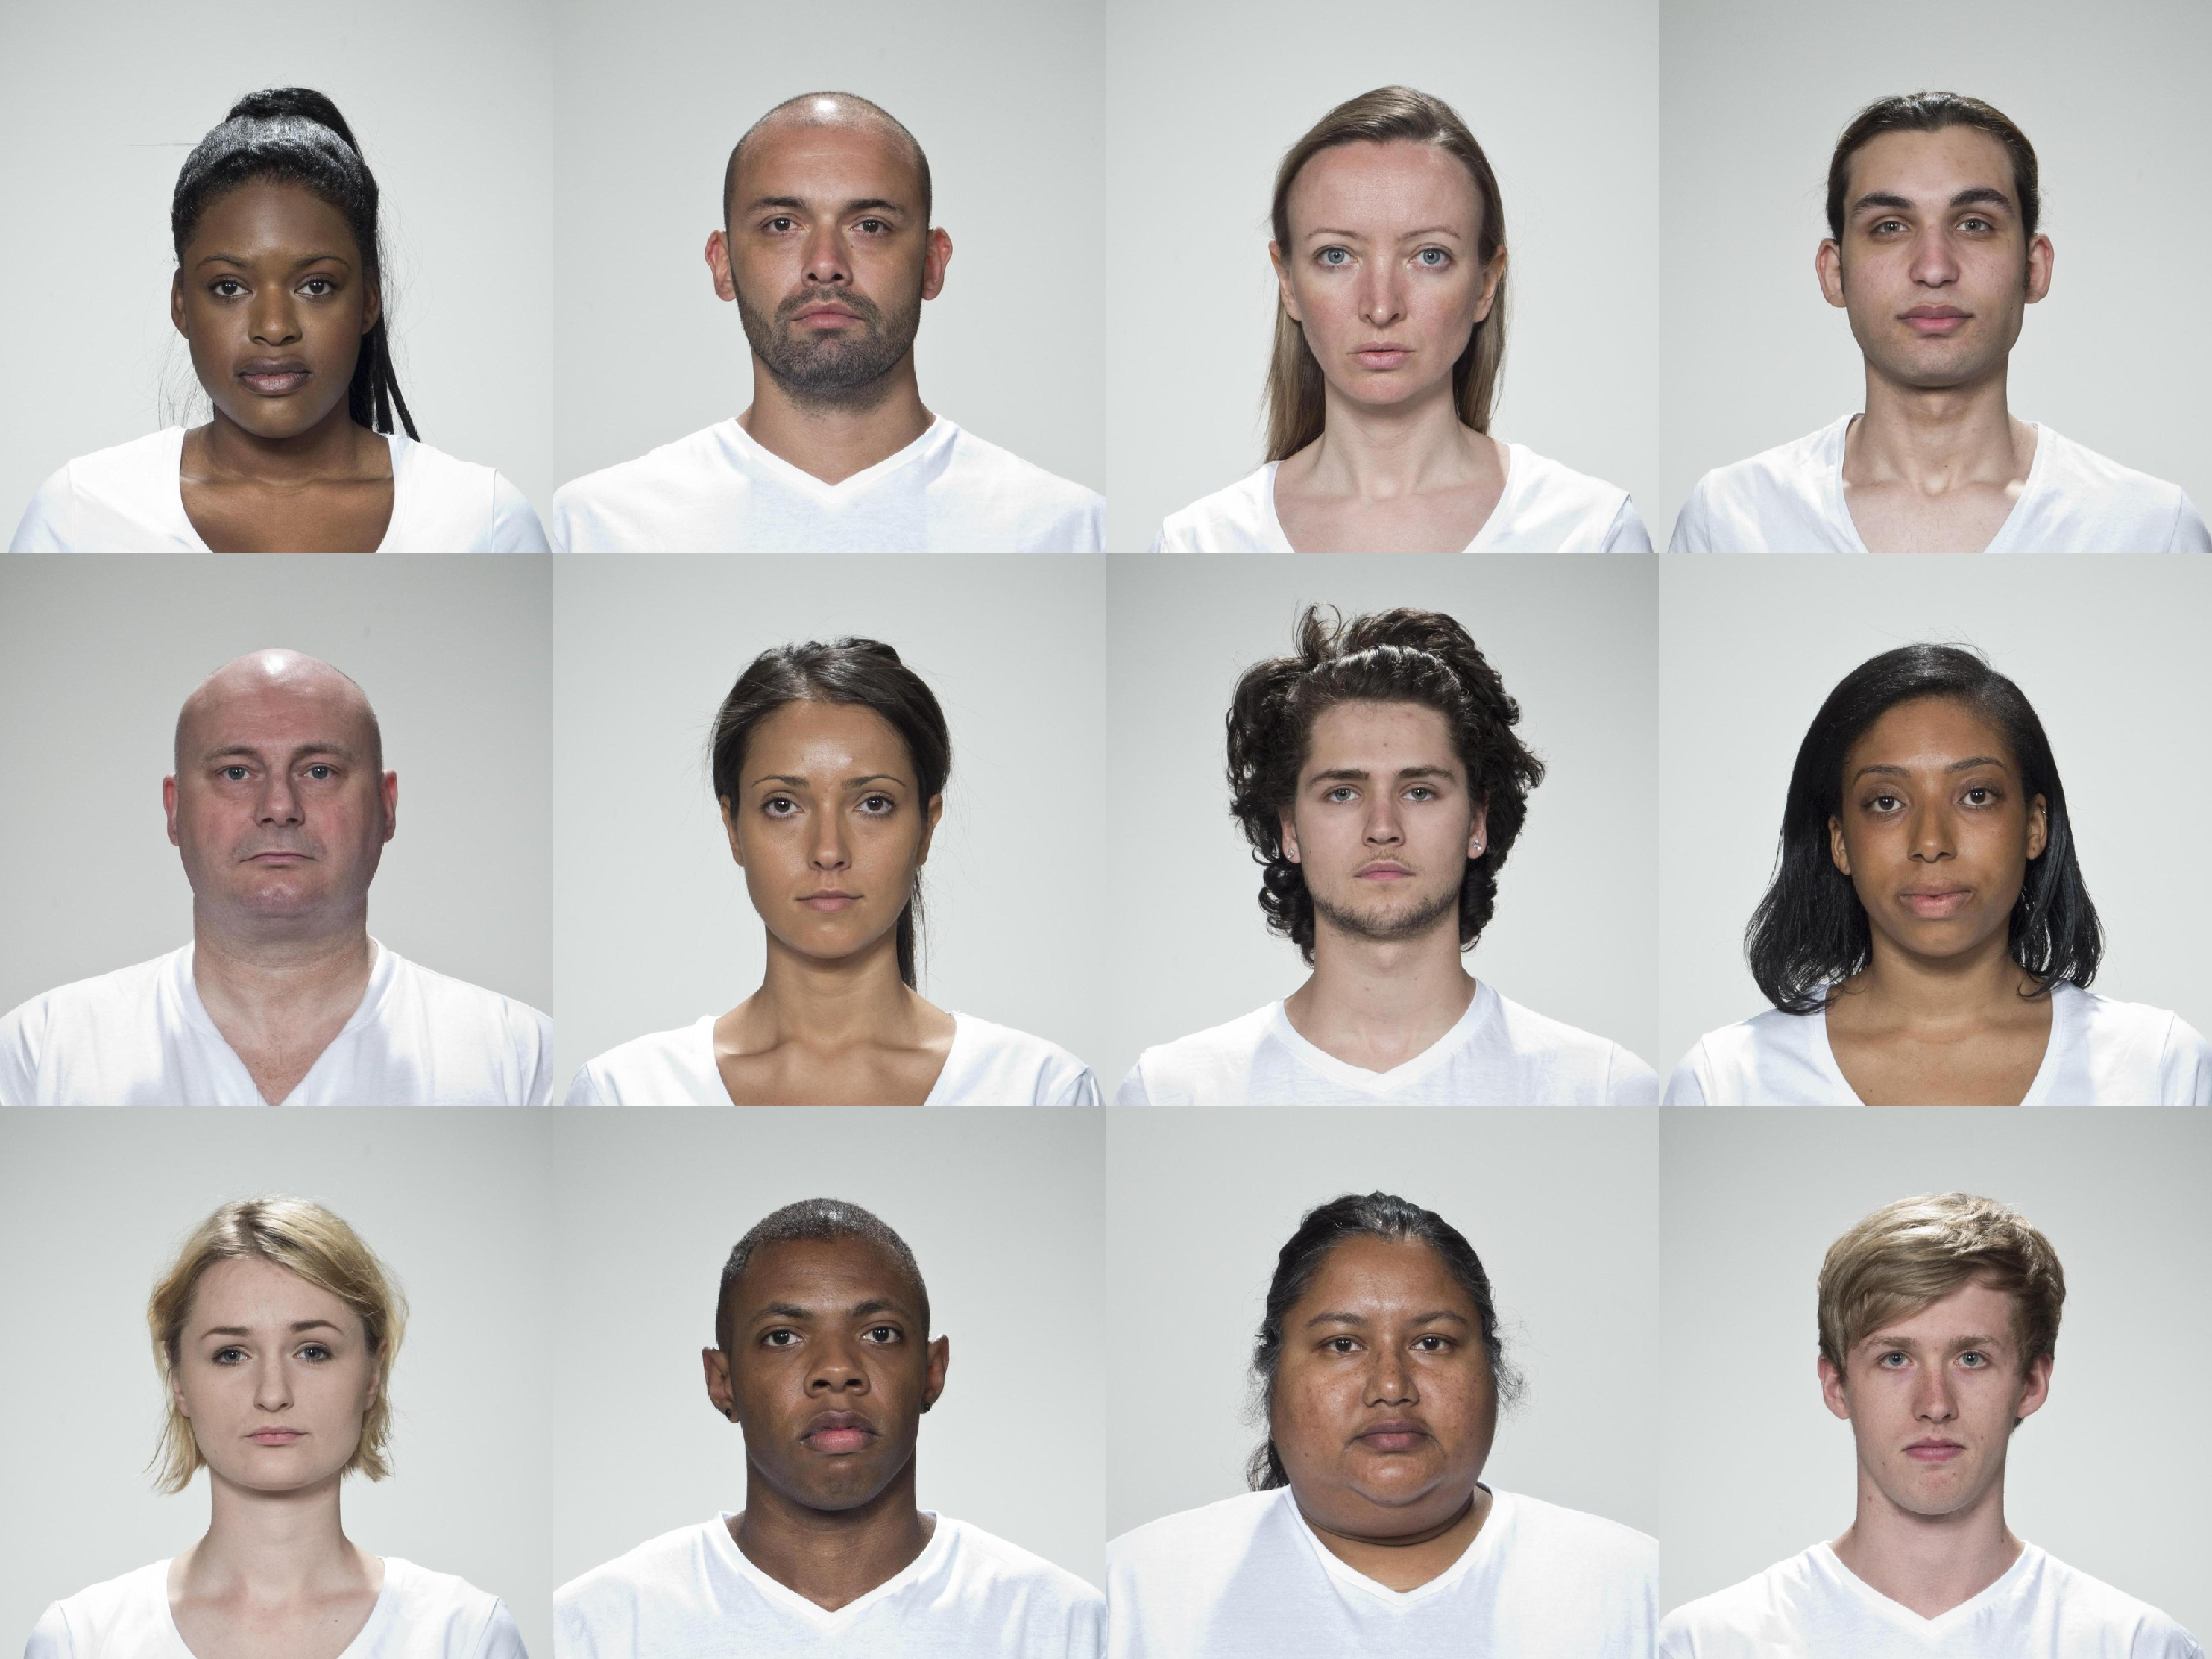
\includegraphics[width=\textwidth]{images/mos_train_set.pdf}\\
        \caption{MOS train set}\label{fig:mos_set_train}
    \end{subfigure}
    \hfill
    \begin{subfigure}[t]{0.19\textwidth}
        \centering
        
\includegraphics[width=\textwidth]{images/mos_test_set.pdf}\\
        \caption{MOS test set}\label{fig:mos_set_test}
    \end{subfigure}
    \caption{Reference images from the MOS set, comprising the selected subjects from the FRLL dataset.}\label{fig:mos_set}
\end{figure}

The steganographic distortions are visible in Fig.~\ref{fig:steganography}, which shows examples of distorted facial images from each method. The distortions are applied to the original images, and the resulting stego images are used for both subjective evaluation and training of the NR-IQA model.

\begin{figure}[ht]
    \centering
    \begin{subfigure}[t]{0.22\textwidth}
        \centering
        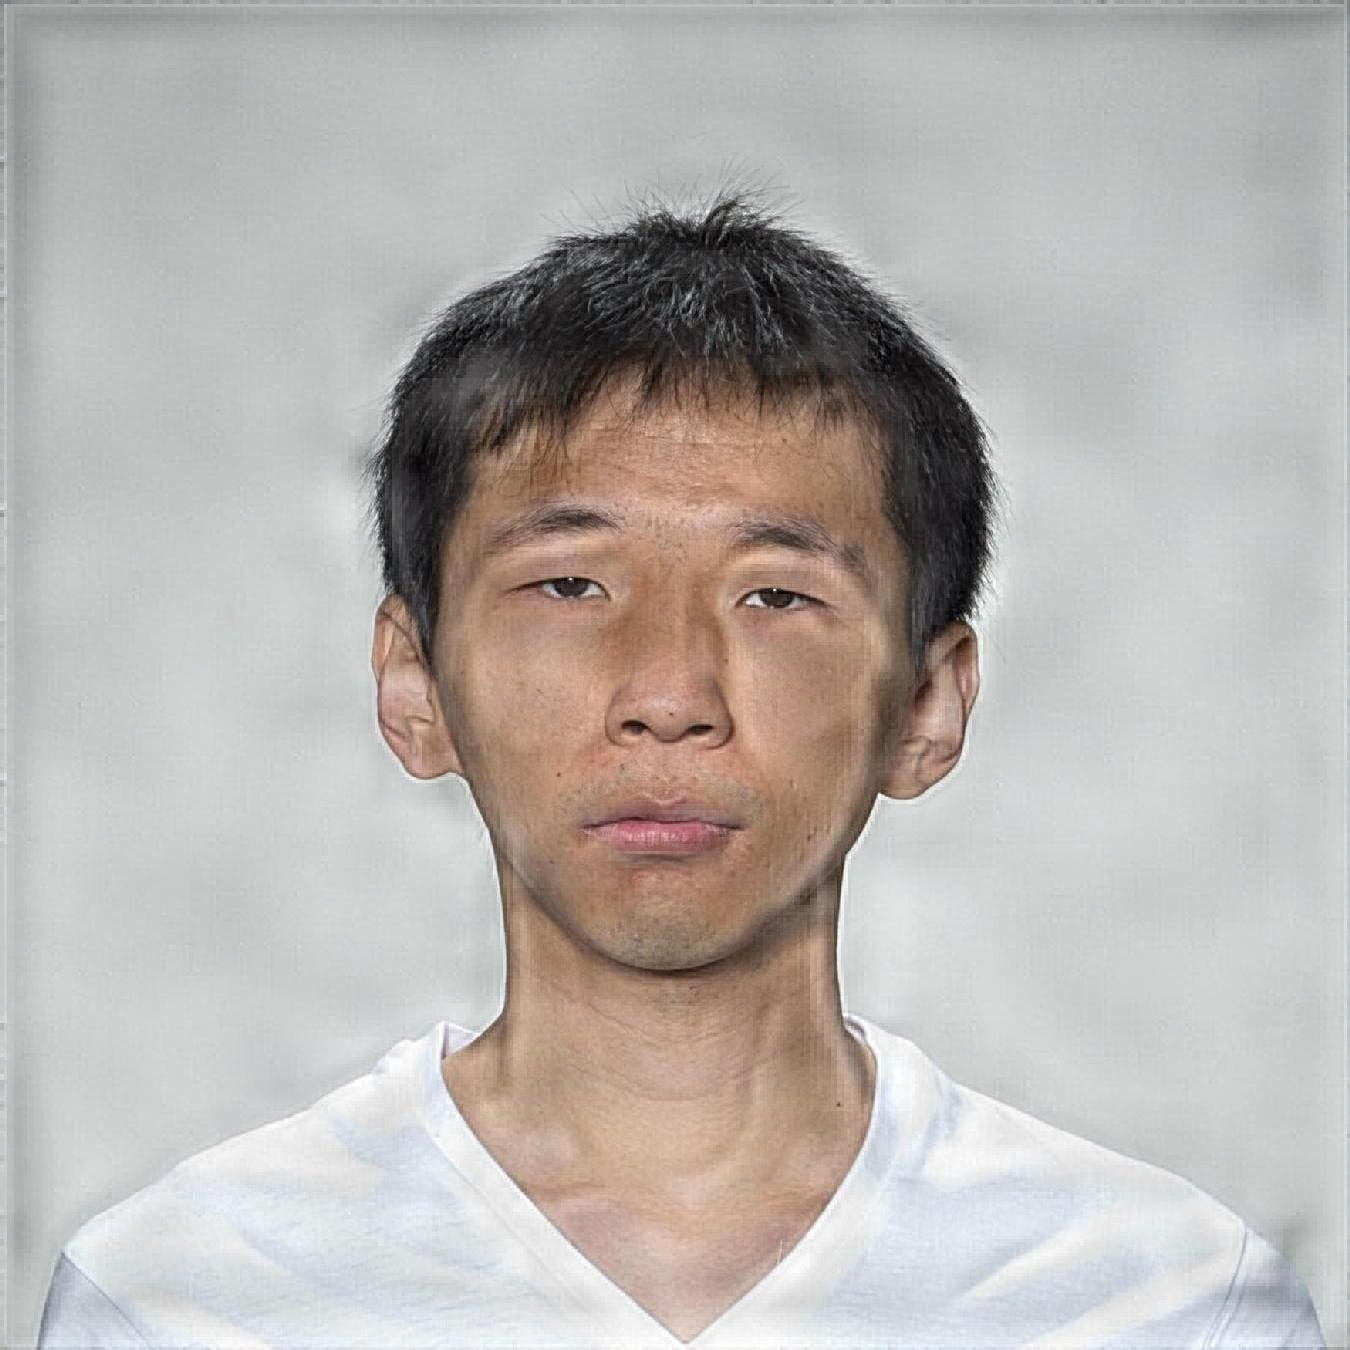
\includegraphics[width=\textwidth]{images/005_StegaStamp_1.4.jpg}\\
        \caption{StegaStamp}\label{fig:steganography_a}
    \end{subfigure}
    \hfill
    \begin{subfigure}[t]{0.22\textwidth}
        \centering
        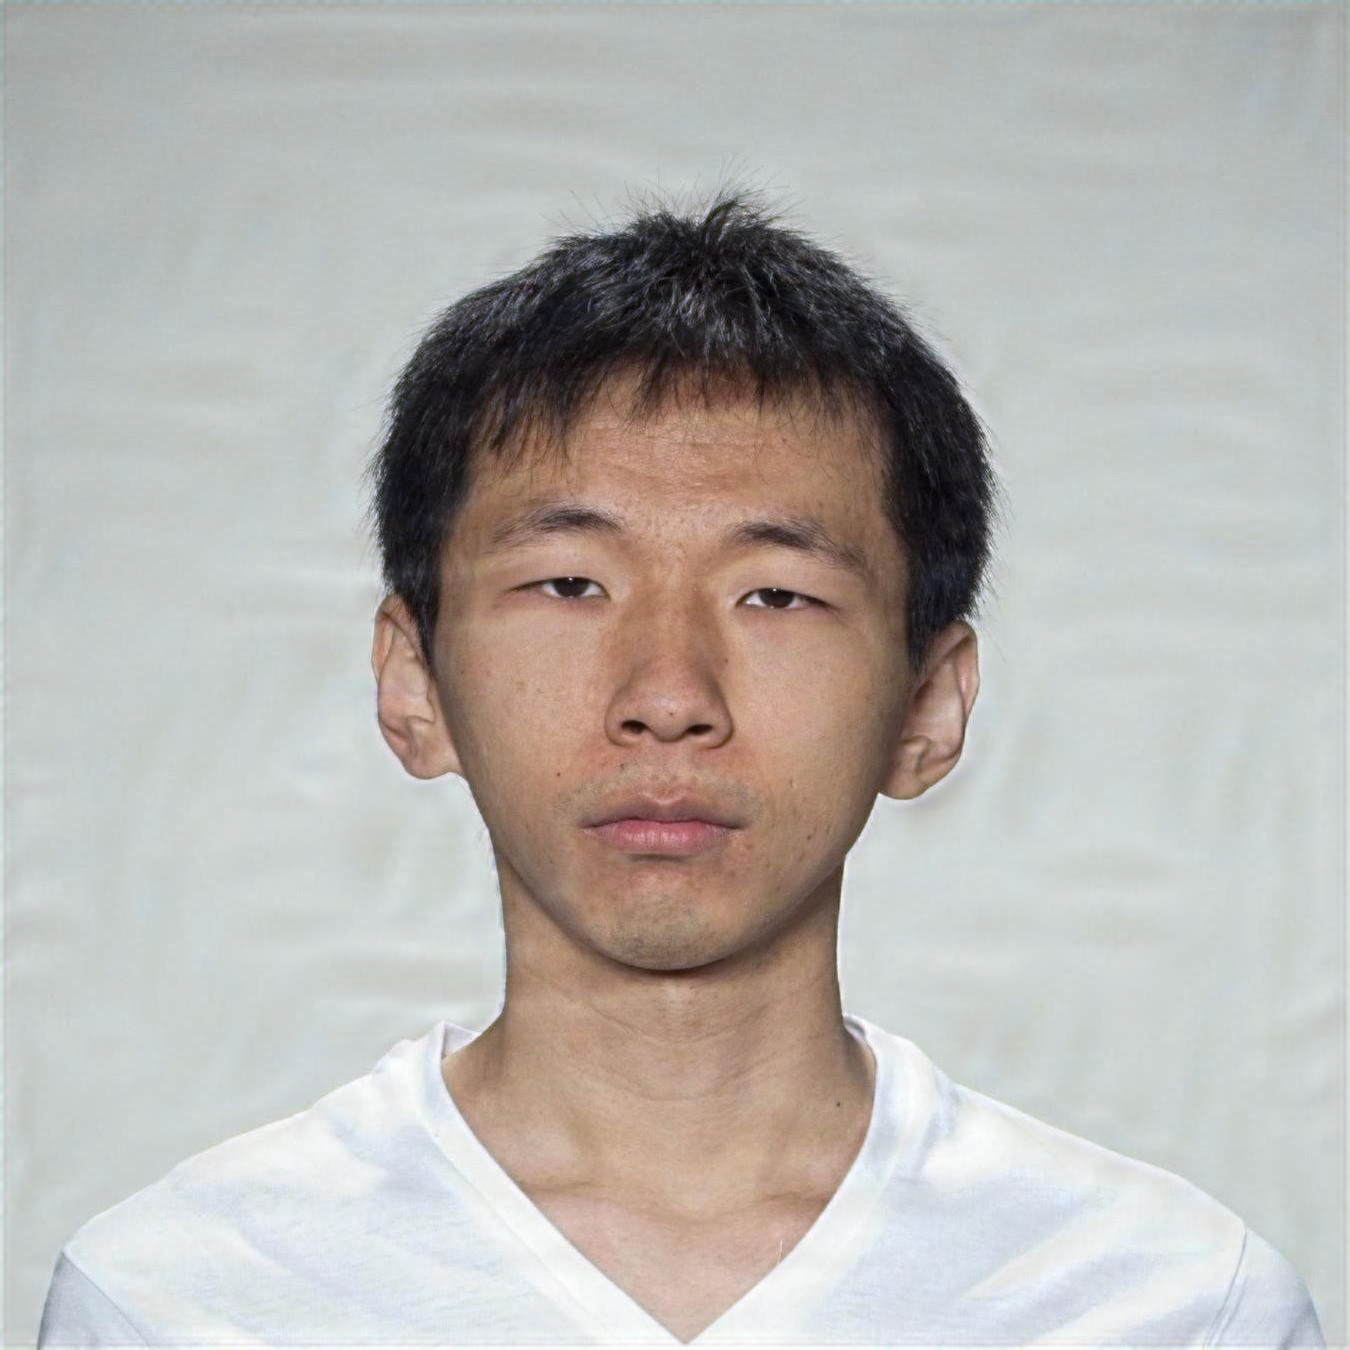
\includegraphics[width=\textwidth]{images/005_CodeFace_1.4.jpg}\\
        \caption{Code\,Face}\label{fig:steganography_b}
    \end{subfigure}
    \hfill
    \begin{subfigure}[t]{0.22\textwidth}
        \centering
        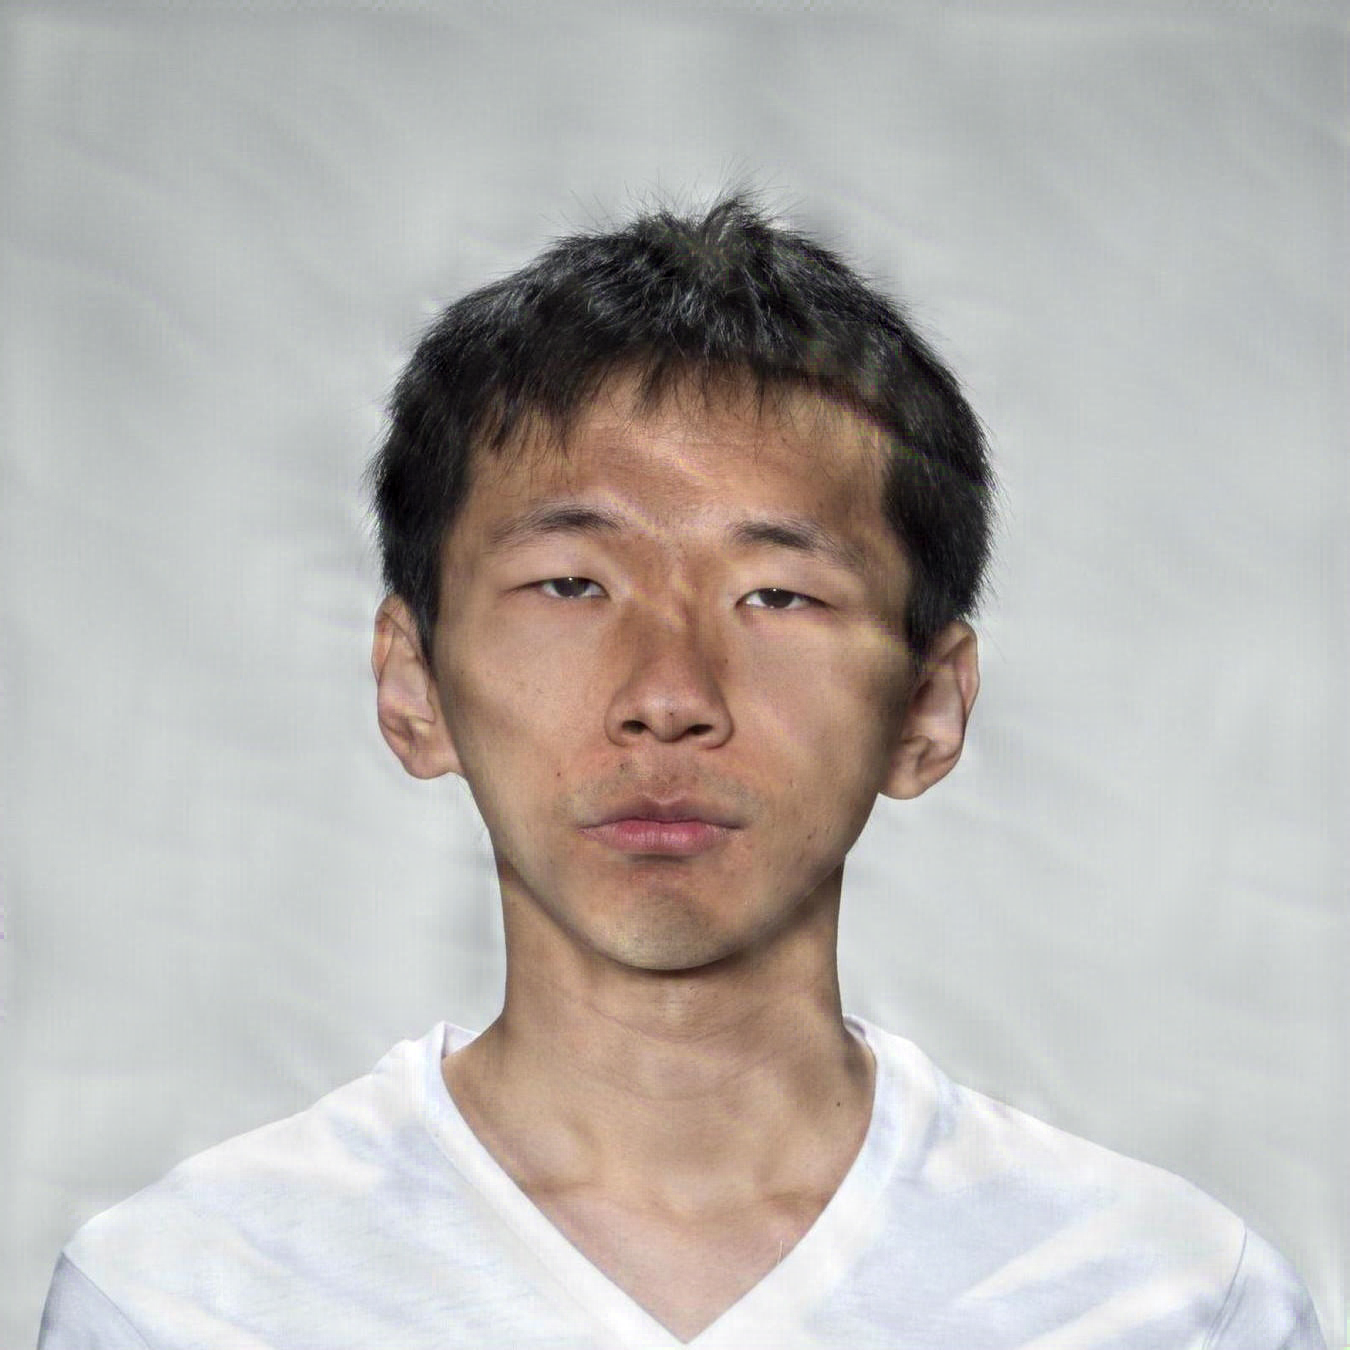
\includegraphics[width=\textwidth]{images/005_RiemStega_1.4.jpg}\\
        \caption{RiemStega}\label{fig:steganography_c}
    \end{subfigure}
    \hfill
    \begin{subfigure}[t]{0.22\textwidth}
        \centering
        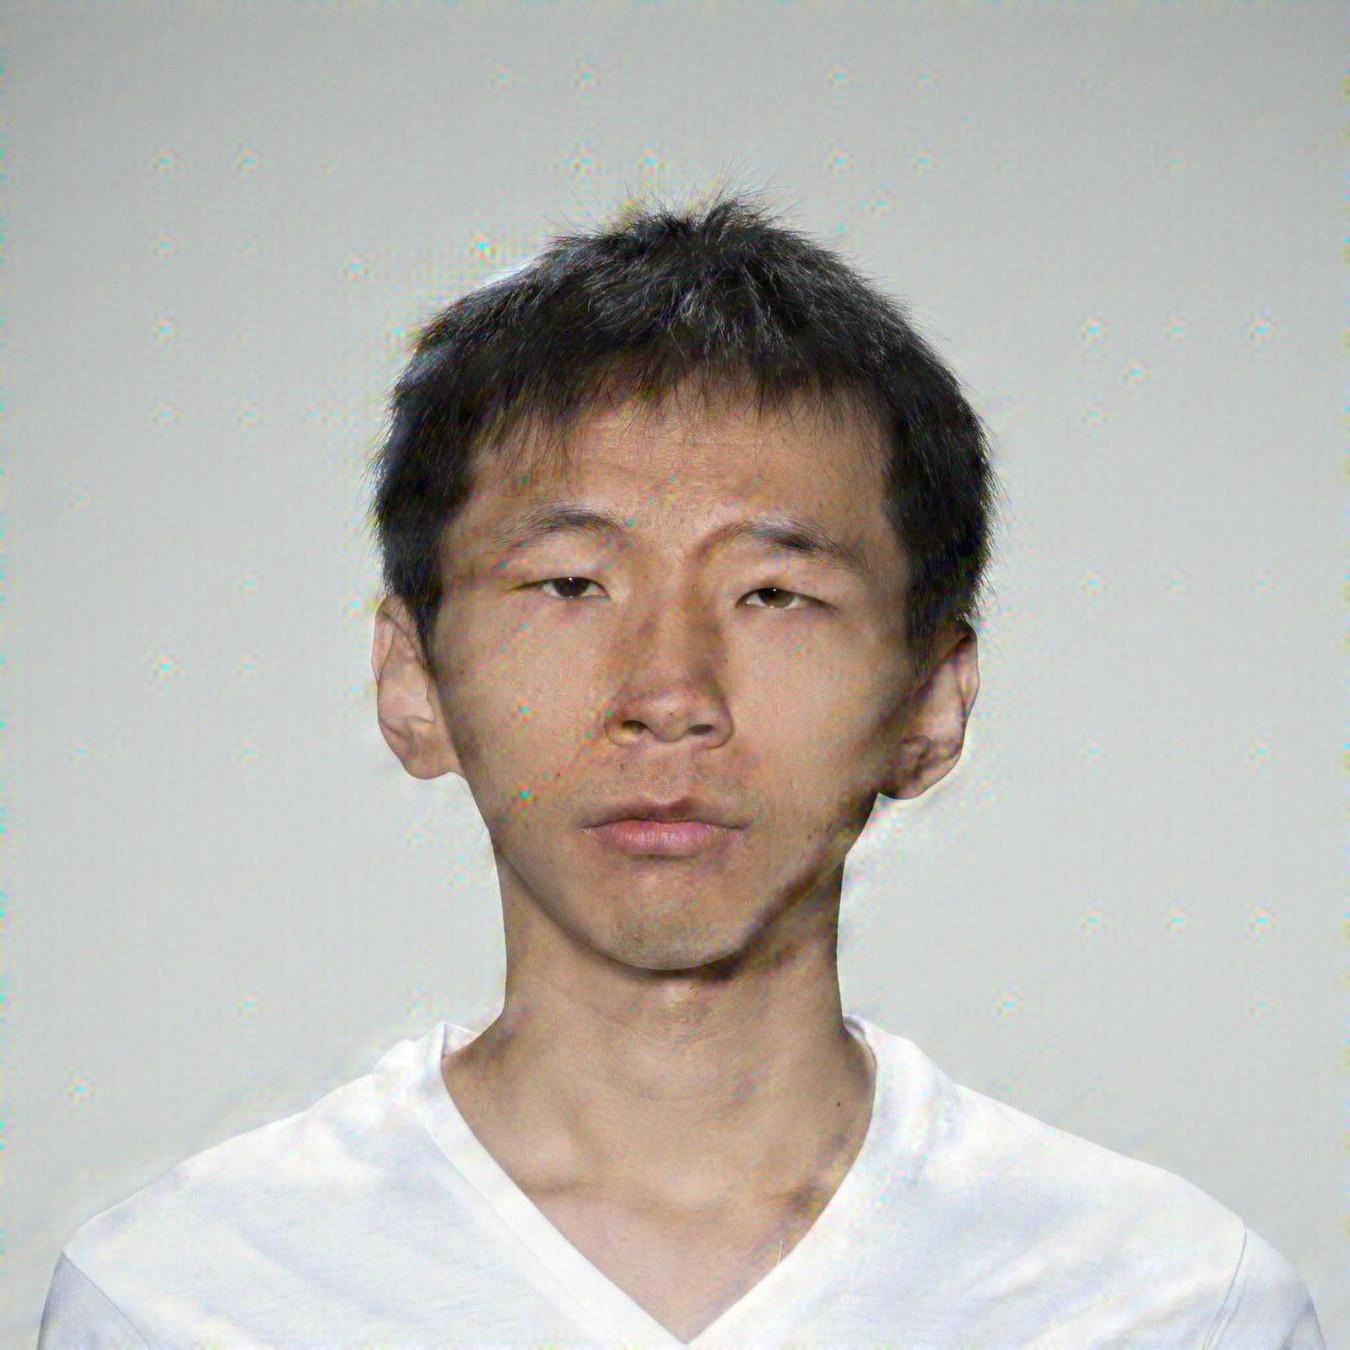
\includegraphics[width=\textwidth]{images/005_StampOne_1.4.jpg}\\
        \caption{StampOne}\label{fig:steganography_d}
    \end{subfigure}
    \caption{Steganographically distorted facial images from each method.}\label{fig:steganography}
\end{figure}

\section{Collection of Subjective Scores}

We followed the ITU-R BT.500--15~\cite{ITU-R-BT500} recommendation and adopted the Single Stimulus (SS) method. The test was implemented using a custom Django web application seen in Fig.~\ref{fig:webapp}. Prior to the test session, participants signed an informed consent form and filled out a registration form providing demographic and environmental information such as age, gender, education, country of origin and ethnicity, and others. Each image was shown individually, with no time limit. Ratings were submitted using a labeled slider, and automatic saving ensured session robustness.

Each image in the MOS set was evaluated approximately 30 times by human observers, resulting in over 14,000 ratings. We had around 200 participants, each session lasted about 22 minutes and included roughly 70 evaluations. Following the session, outlier observers were identified and removed using both Kurtosis-based and correlation-based post-screening methods described in ITU-R BT.500--15~\cite{ITU-R-BT500}, resulting in the exclusion of one participant.

\begin{figure}
    \centering
    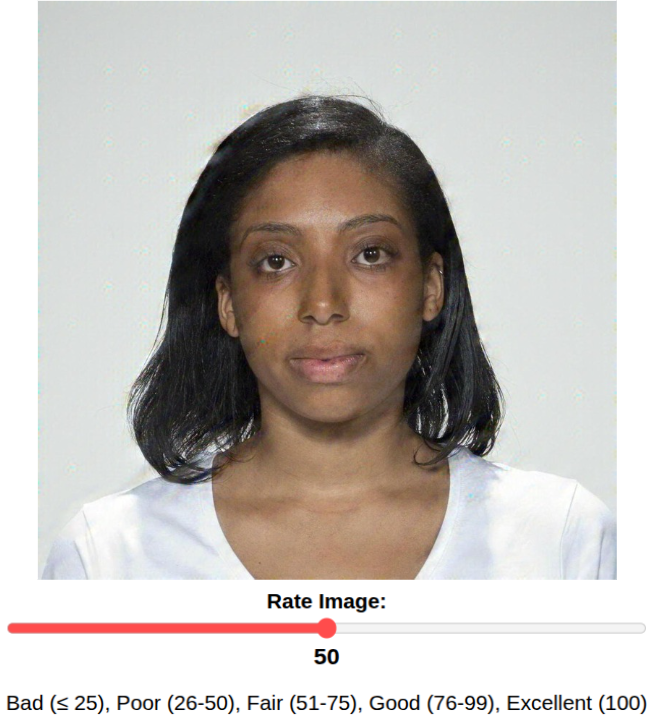
\includegraphics[width=0.32\textwidth]{images/webapp_test.png}
    \caption{Django-based webapp created for the Single Stimulus test.}\label{fig:webapp}
\end{figure}

The database was implemented using the Django web framework, which provides an object-relational mapping (ORM) layer that directly maps Python model classes to database tables. The ORM also enforces data integrity constraints and simplifies querying for statistical analysis. The database backend used was PostgreSQL.

The database schema was designed to ensure structured storage and traceability of all subjective quality evaluation data. Fig.~\ref{fig:db_conceptual} presents the conceptual data model, which defines the main entities and their relationships. The profile entity stores participant metadata, including age, gender, education, ethnicity, country, and device used. The ss\_session entity models individual test sessions and is linked to both the participant profile and the dataset being evaluated. The image entity encodes each image's filename, associated distortion type (distortion\_name), and distortion level (distortion\_level). The test entity stores individual subjective ratings, including the precise timestamp of submission, linked to both the session and the image presented. An auxiliary user\_feedback entity captures optional, anonymous, observer comments and critiques.

The physical implementation of this schema, shown in Fig.~\ref{fig:db_physical}, is realized as a relational database with explicit foreign key constraints to ensure referential integrity. The dataset\_id and profile\_id fields in ss\_session formally enforce the linkage to specific datasets and participants. The test table connects each subjective rating to its session (ss\_session\_id) and image (image\_id), enabling consistent aggregation of ratings into a statistical descriptors such as MOS and confidence intervals per image and per distortion level. The relational model also facilitates efficient querying for downstream statistical analysis and supports reproducibility of the experimental protocol in line with ITU-R BT.500-15 recommendations.

\begin{figure}
    \centering
    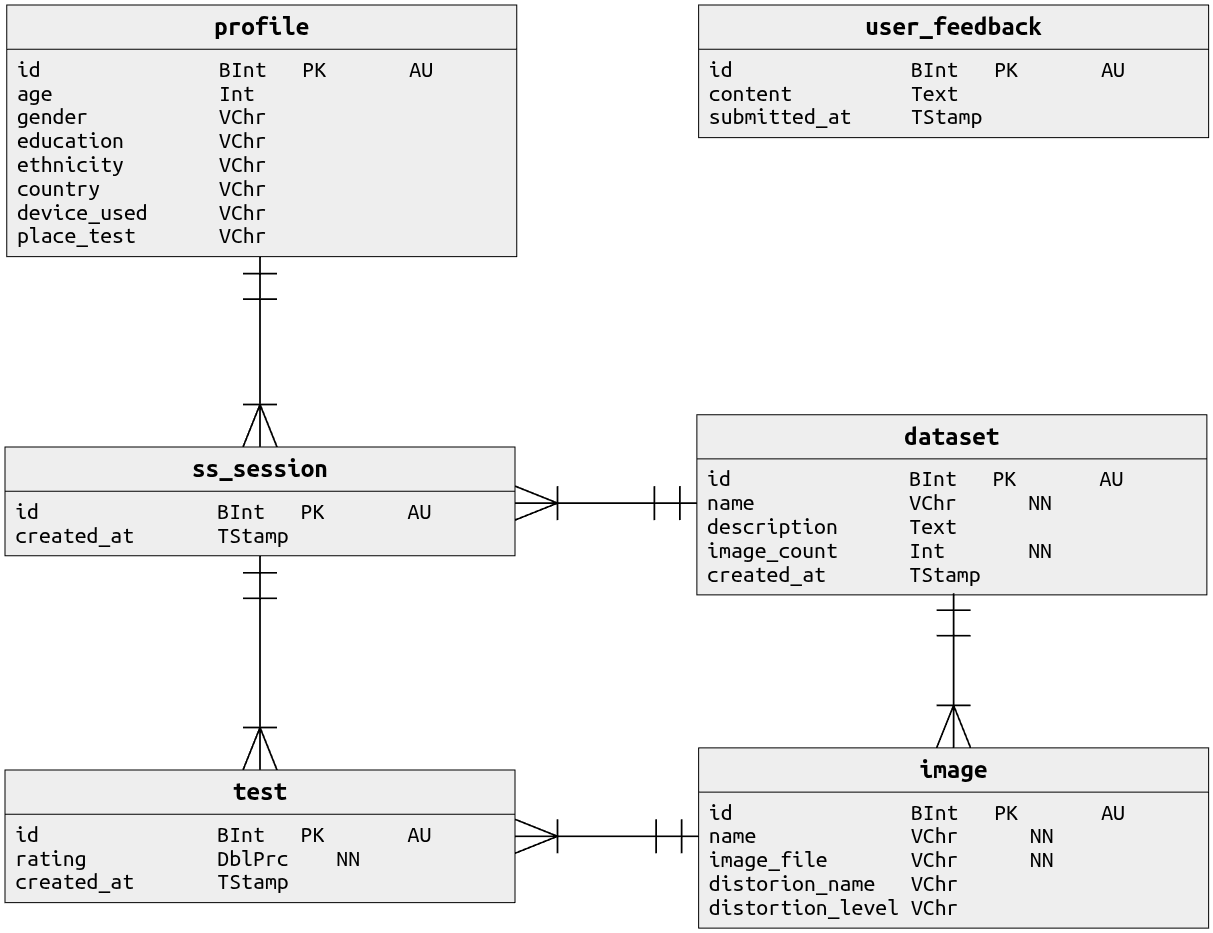
\includegraphics[width=0.8\textwidth]{images/db_conceptual.png}
    \caption{Conceptual database schema.}\label{fig:db_conceptual}
\end{figure}

\begin{figure}
    \centering
    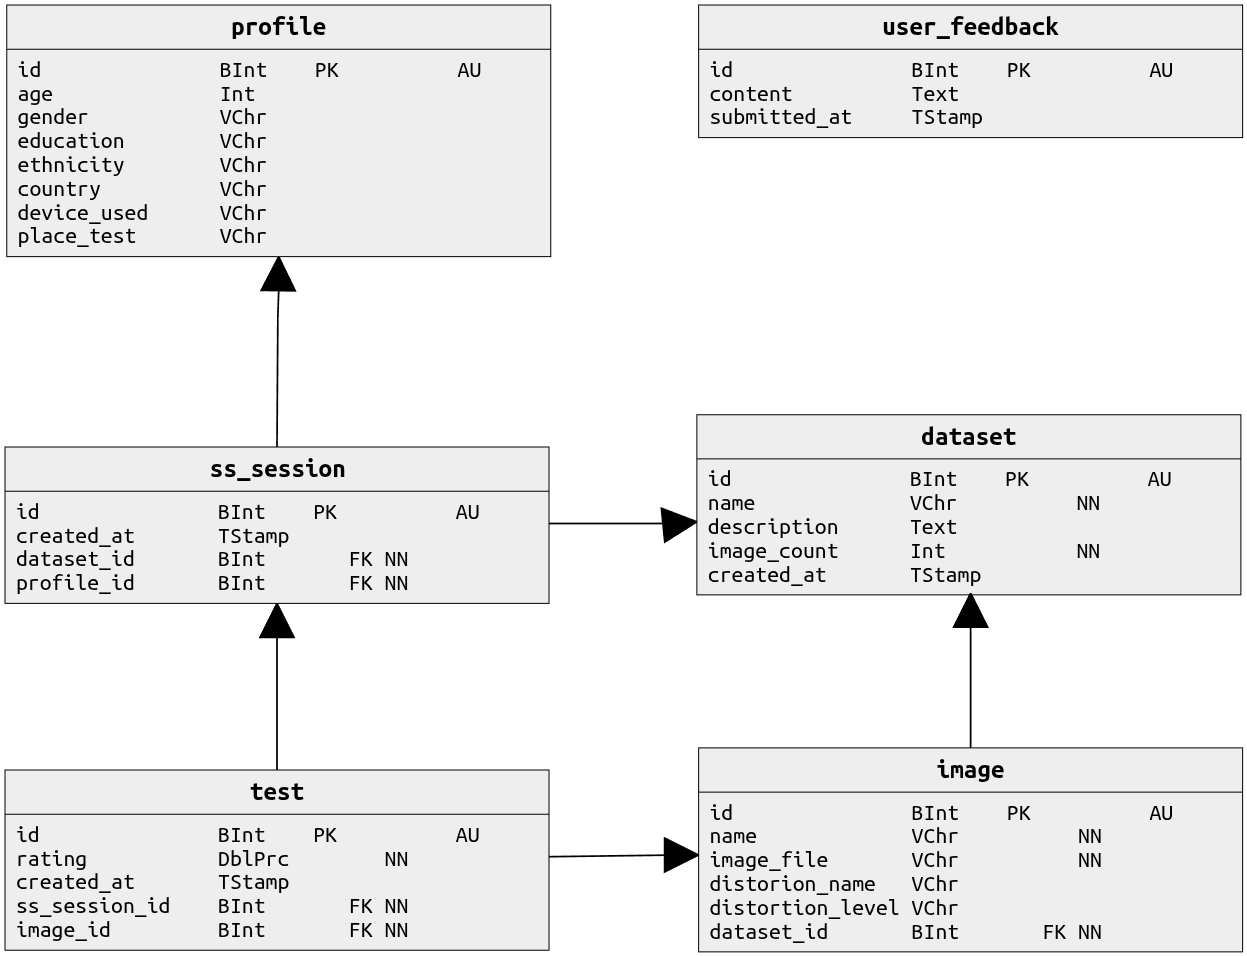
\includegraphics[width=0.8\textwidth]{images/db_physical.png}
    \caption{Physical database schema.}\label{fig:db_physical}
\end{figure}


\section{Debiasing of Subjective Scores}

To correct for demographic bias in the subjective scores, we followed a procedure inspired by prior work on bias correction in perceptual tasks~\cite{clapes2018apparent}, where we applied a residualization method based on linear modeling. An ordinary least squares (OLS) regression was fit to the MOS values, using observer and image attributes, and their pairwise interactions as categorical predictors. The fitted bias components were subtracted from the original scores, and the residuals were mean-centered to preserve the global score distribution. As shown in Table~\ref{tab:anova}, several factors exhibit statistically significant effects on the MOS prior to residualization, notably observer and subject ethnicity. After applying the residualization procedure, these effects disappear, as confirmed by an ANOVA test showing no significant impact from any individual factor. The corrected MOS labels are then used as ground truth in all supervised stages of the pipeline to ensure fairness and reduce the influence of socially conditioned priors.

\begin{table}
    \centering
    \caption{ANOVA~\cite{ross2017one} results for observer and image attributes. Before debiasing, several factors show statistically significant effects on MOS, p-value $< 0.05$.\@ After residualization, all main effects show no significant impact, confirming the effectiveness of the debiasing procedure.}\label{tab:anova}
    \begin{tabular}{lcc}
        \hline % chktex 44
        Factor & p-value & p-value (residualized) \\
        \hline % chktex 44
        Observer gender                             & 0.022                 & 0.9930 \\
        Observer ethnicity                          & $8.44 \times 10^{-4}$ & 1 \\
        Subject gender                              & $1.60 \times 10^{-3}$ & 0.9722 \\
        Subject ethnicity                           & $7.36 \times 10^{-3}$ & 1 \\
        Observer gender $\times$ Subject gender     & 0.6417              & 0.6417 \\
        Observer ethnicity $\times$ Subject ethnicity & 0.0582              & 0.0582 \\
        \hline % chktex 44
    \end{tabular}
\end{table}

\section{Correlation of FR-IQA Metrics with Human Perception}

We compute 40 FR-IQA scores for each distorted image in the dataset and compare them against the corresponding MOS, as seen in Fig.~\ref{fig:mos_vs_iqa}. Several metrics exhibit strong linear trends with MOS, while others are poorly aligned or even negatively correlated. For a detailed description of these metrics, we refer the reader to~\cite{shahrukh2019survey}.



\begin{figure}
    \centering
    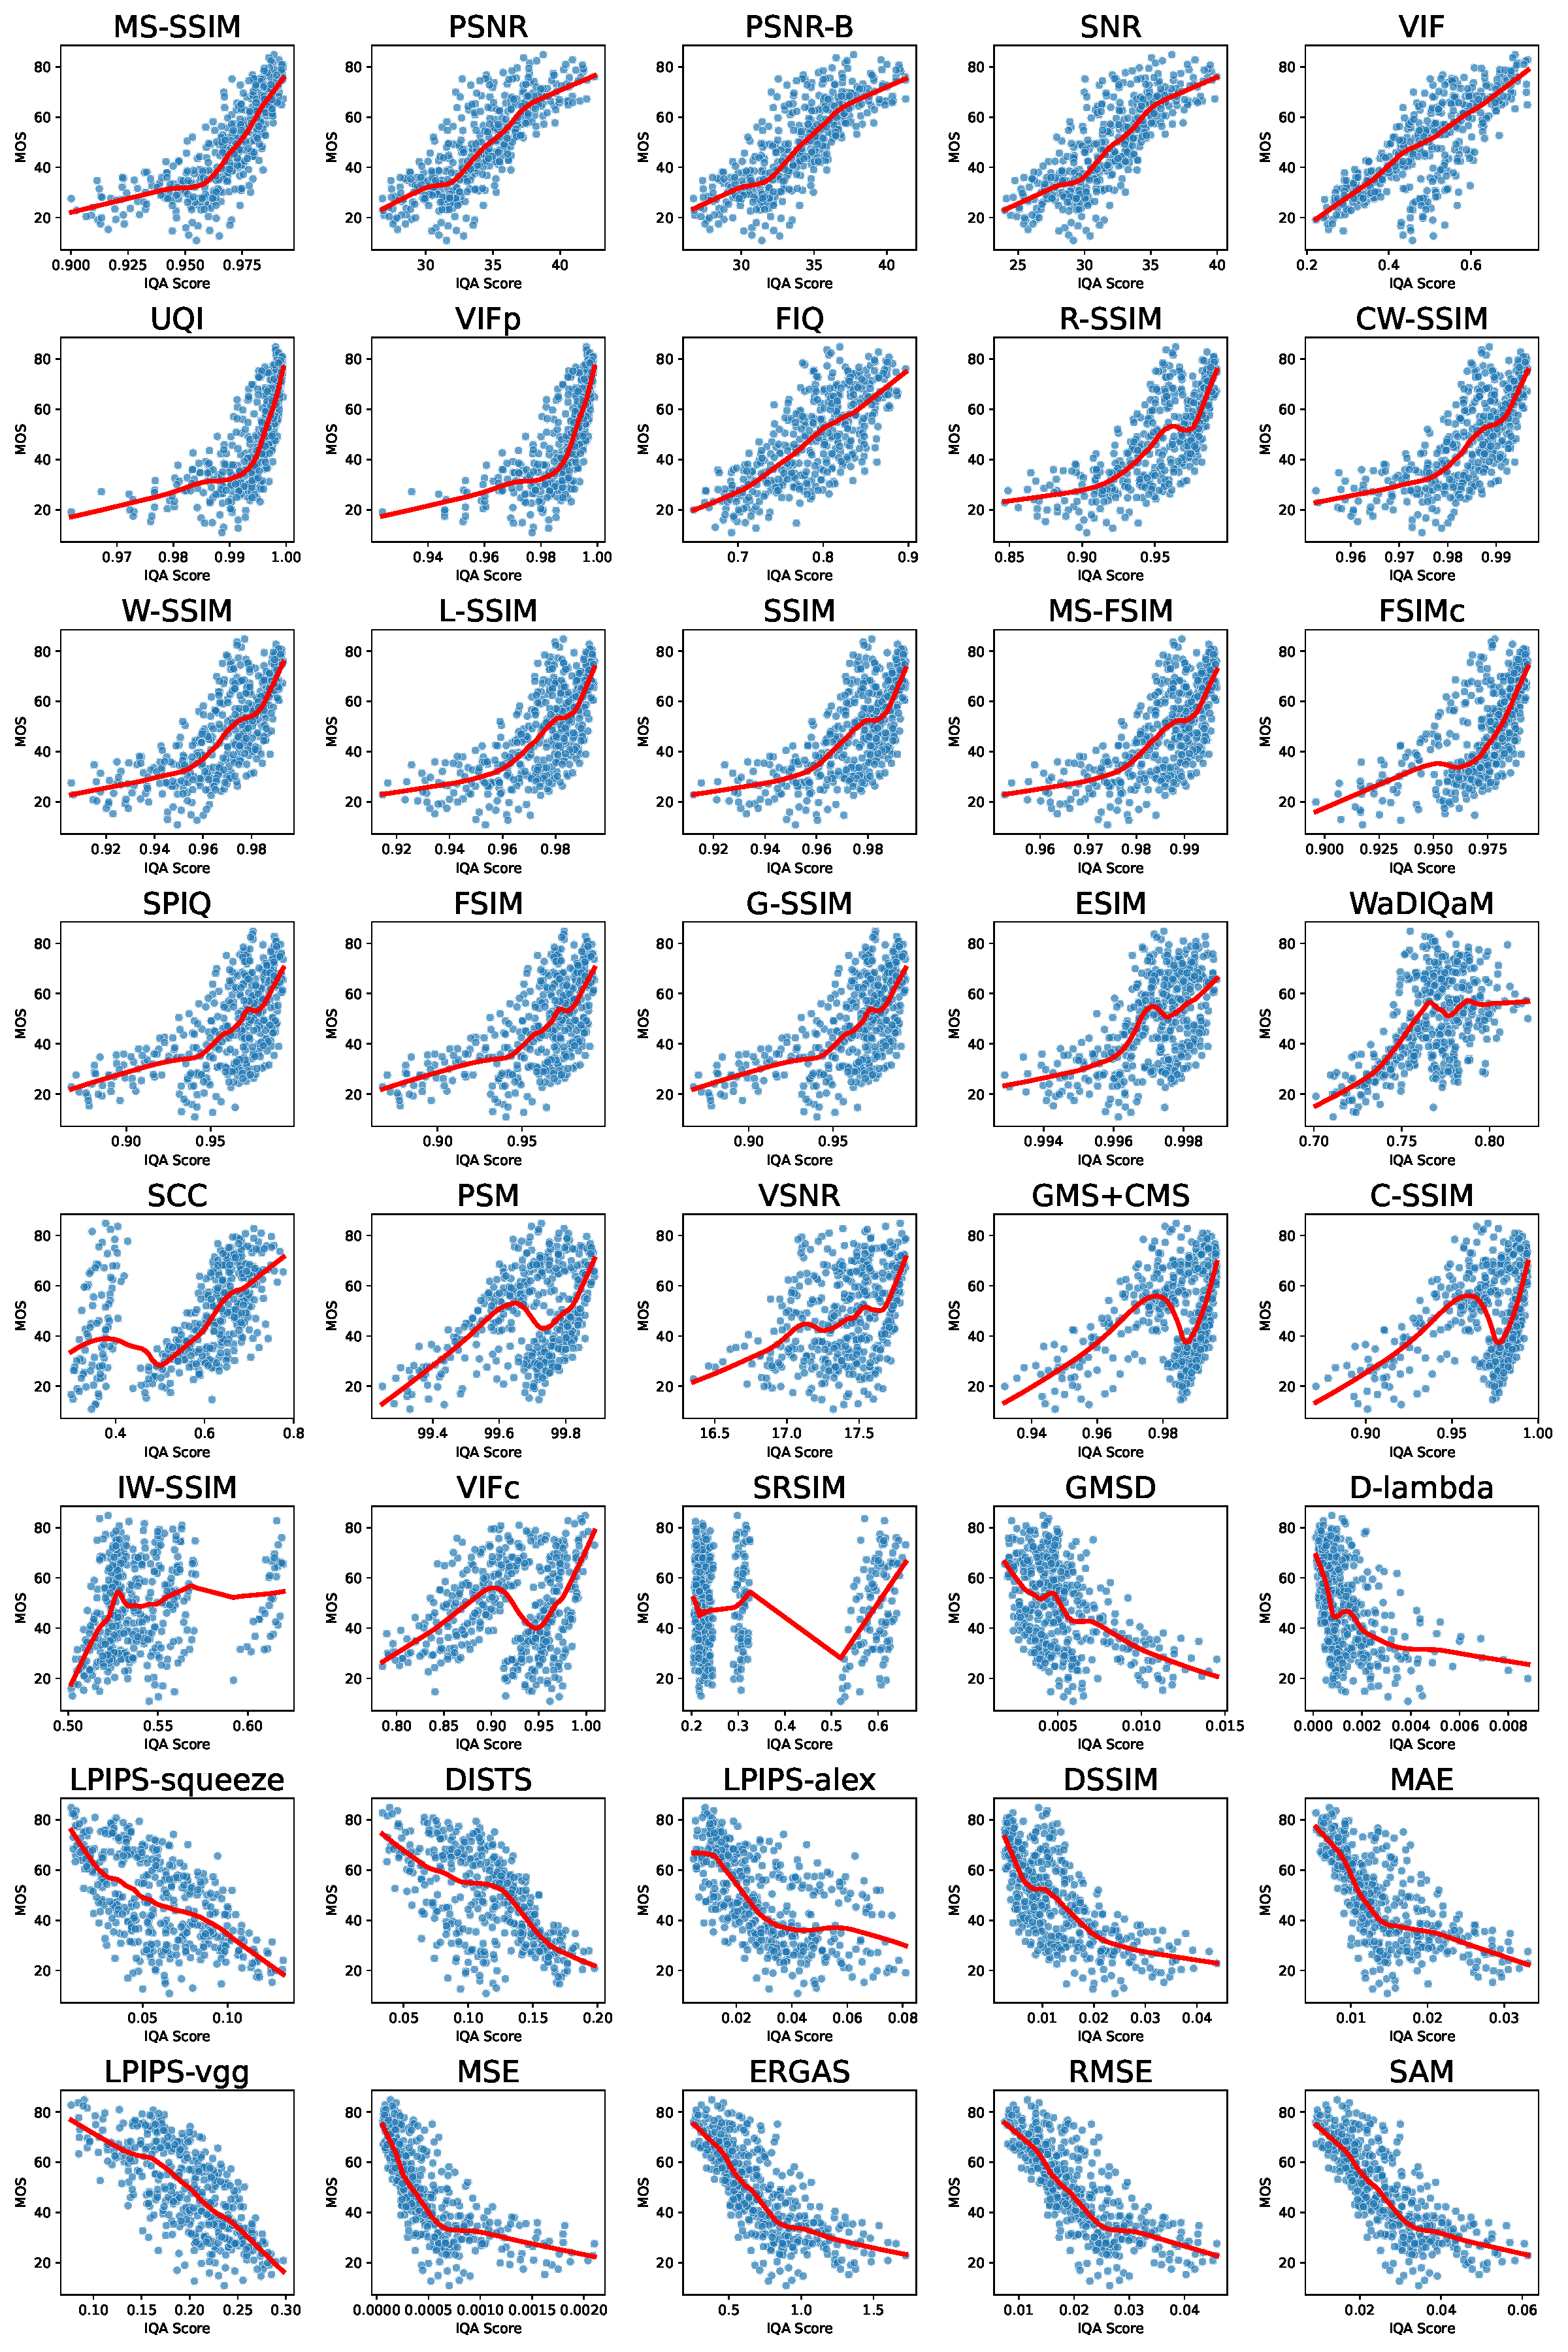
\includegraphics[width=0.90\linewidth]{images/mos_vs_iqa_grid.pdf}
    \caption{Scatter plots illustrating the relationship between MOS and 40 individual full-reference IQA metrics. The red line represents a smoothed local trend curve.}\label{fig:mos_vs_iqa}
\end{figure}

\section{Fusion of FR-IQA Metrics for Pseudo-MOS Estimation}

To identify which metrics align best with human perception, we compute both the Pearson Linear Correlation Coefficient (PLCC) and the Spearman Rank-Order Correlation Coefficient (SRCC)~\cite{plcc-srcc} which respectively quantify the linearity and monotonicity of the relationship between metric scores and MOS.\@ To determine the appropriate number of metrics to retain for fusion, we applied Singular Value Decomposition (SVD) and the Picard criterion~\cite{hansen1998picard}. Metrics are first ranked by the average of their PLCC and SRCC with MOS.\@ After normalizing the feature matrix, SVD revealed that six components capture 95\% of the total variance, as shown in Fig.~\ref{fig:svd_analysis}a, indicating an optimal dimensionality of $k=6$.

To validate this truncation point, we examined the Picard plot in Fig.~\ref{fig:svd_analysis}b, which compares singular values with the target projections. The stable ratio in the tail confirms that six components provide a good balance between expressiveness and stability. This supports a compact, informative subset of FR-IQA metrics.

\begin{figure}[ht]
    \centering
    \begin{minipage}[t]{0.48\textwidth}
        \centering
        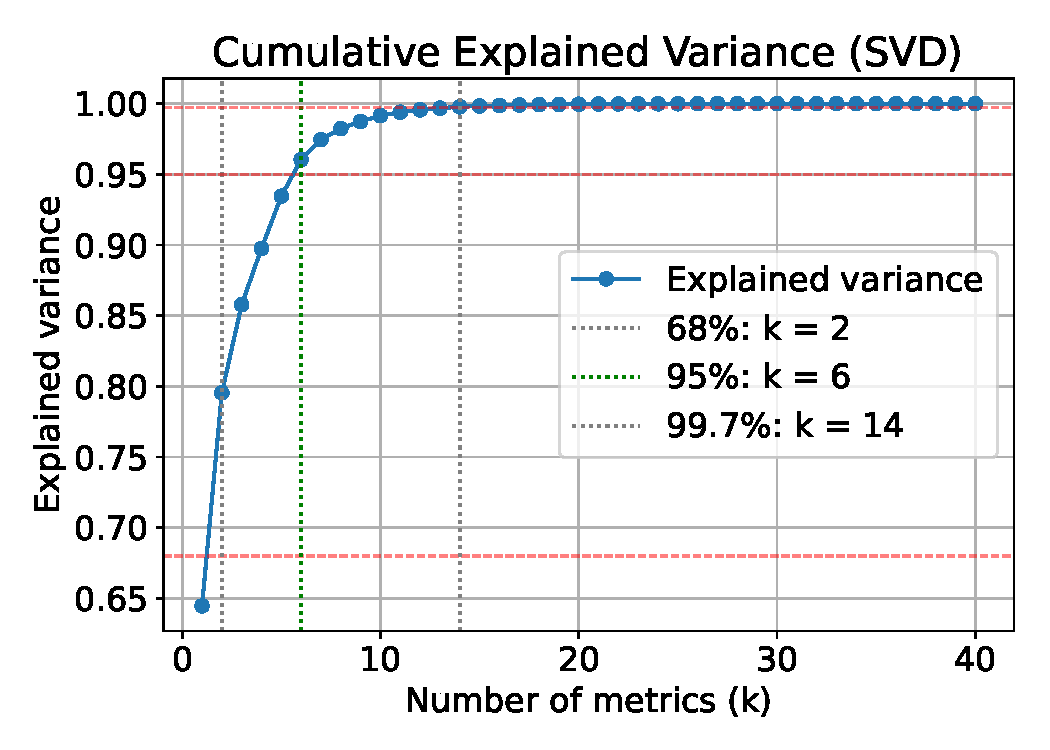
\includegraphics[width=\linewidth]{images/variance.pdf}
        \textbf{(a)} Cumulative variance explained by SVD components.
    \end{minipage}
    \hfill
    \begin{minipage}[t]{0.48\textwidth}
        \centering
        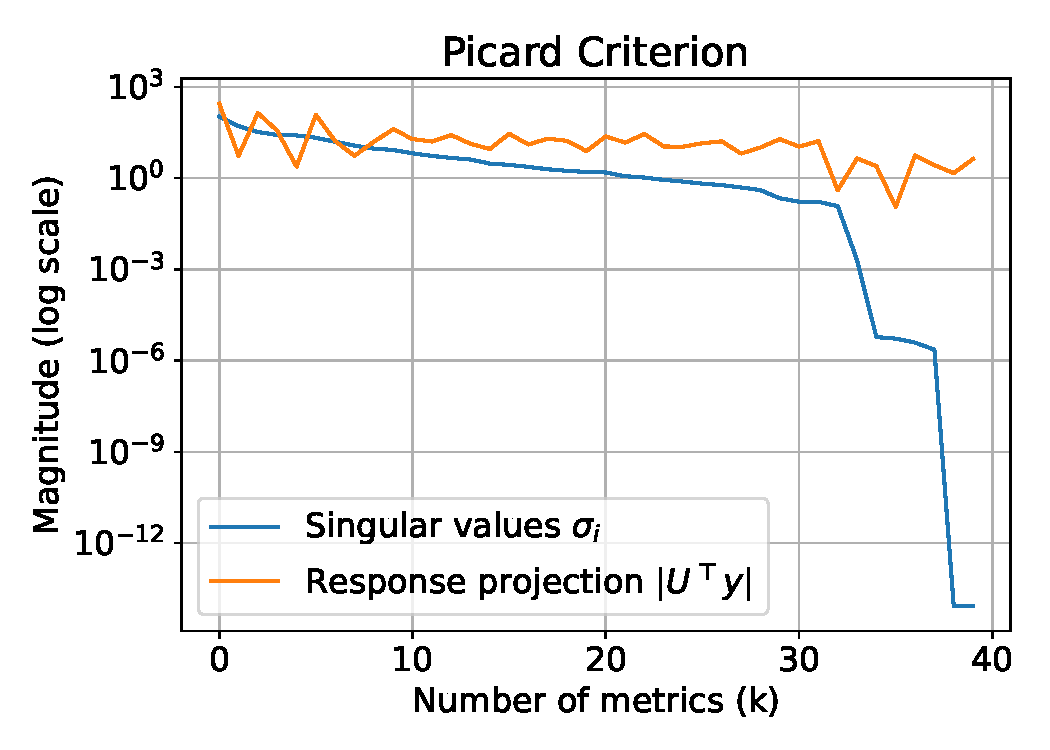
\includegraphics[width=\linewidth]{images/picard.pdf}
        \textbf{(b)} Magnitude of singular values and projected response.
    \end{minipage}
    \caption{SVD-based analysis of the FR metric space. The cumulative explained variance (a) guides the choice of dimensionality, while the Picard criterion (b) illustrates stability near $k=6$.}\label{fig:svd_analysis}
\end{figure}

After selecting the top $k = 6$ FR-IQA metrics, we trained a diverse set of supervised regressors to map these features to subjective MOS scores. The models included both linear and non-linear types:

\begin{itemize}
    \item Linear models: Linear Regression~\cite{linearregression}, Ridge Regression~\cite{ridgeregression}, Bayesian Ridge~\cite{bayesianridge}, ElasticNet~\cite{elasticnet}.
    \item Kernel-based: Support Vector Regression~\cite{svr} (SVR).
    \item Ensembles: Random Forest~\cite{randomforest}, Extra Trees~\cite{ensembles}, Gradient Boosting~\cite{gradboosting}, HistGradientBoosting~\cite{histboost}.
    \item Boosted Trees: XGBoost\cite{xgboost}, LightGBM~\cite{lightgbm}, CatBoost~\cite{catboost}.
\end{itemize}

Each regressor was trained using five-fold cross-validation with an exhaustive grid search over predefined hyperparameter spaces. The best model, CatBoost, optimal configuration was: depth = 8, iterations = 500, learning rate = 0.05, and $L_2$ regularization = 1. This trained regressor is then applied to the unlabeled portion of the dataset (3,132 distorted images), generating pseudo-MOS.\@

\section{Training a No-Reference IQA Model from Pseudo-MOS}

To enable NR quality prediction, we train a deep regression model end-to-end using pseudo-MOS scores as targets. The architecture is based on a ResNet-18 backbone~\cite{resnet} pretrained on ImageNet~\cite{imagenet}, with its final classification layer replaced by a lightweight multi-layer perceptron (MLP) regressor~\cite{bayesianridge}. All layers are fine-tuned during training to learn perceptual quality representations specific to our task. The training set consists of distorted facial images paired with either pseudo-MOS, from the FR fusion, or real MOS labels, when available. The model is optimized using MSE and evaluated on the, disjoint, MOS test set of labeled images. Once trained, the model infers image quality solely from the distorted input, enabling NR assessment aligned with human perception.


\section{Results}

\subsection{Correlation of Individual IQA Metrics with Human Perception}

The correlation analysis between individual FR-IQA metrics and human-rated MOS revealed substantial variability in performance. As shown in Fig.~\ref{fig:mos_vs_iqa}, several metrics exhibit strong linear trends with MOS, while others are poorly aligned or even negatively correlated. To quantify this, we ranked all 41 metrics based on the average of their PLCC and SRCC.\@

Fig.~\ref{fig:ranking} presents this ranking, highlighting that metrics such as PSNR, PSNR-B~\cite{ma2011psnr}, and MS-SSIM~\cite{wang2003multiscale} show the highest alignment with subjective opinion, while others, such as SRSIM~\cite{wang2004image}, diverge significantly.


\begin{figure}
    \centering
    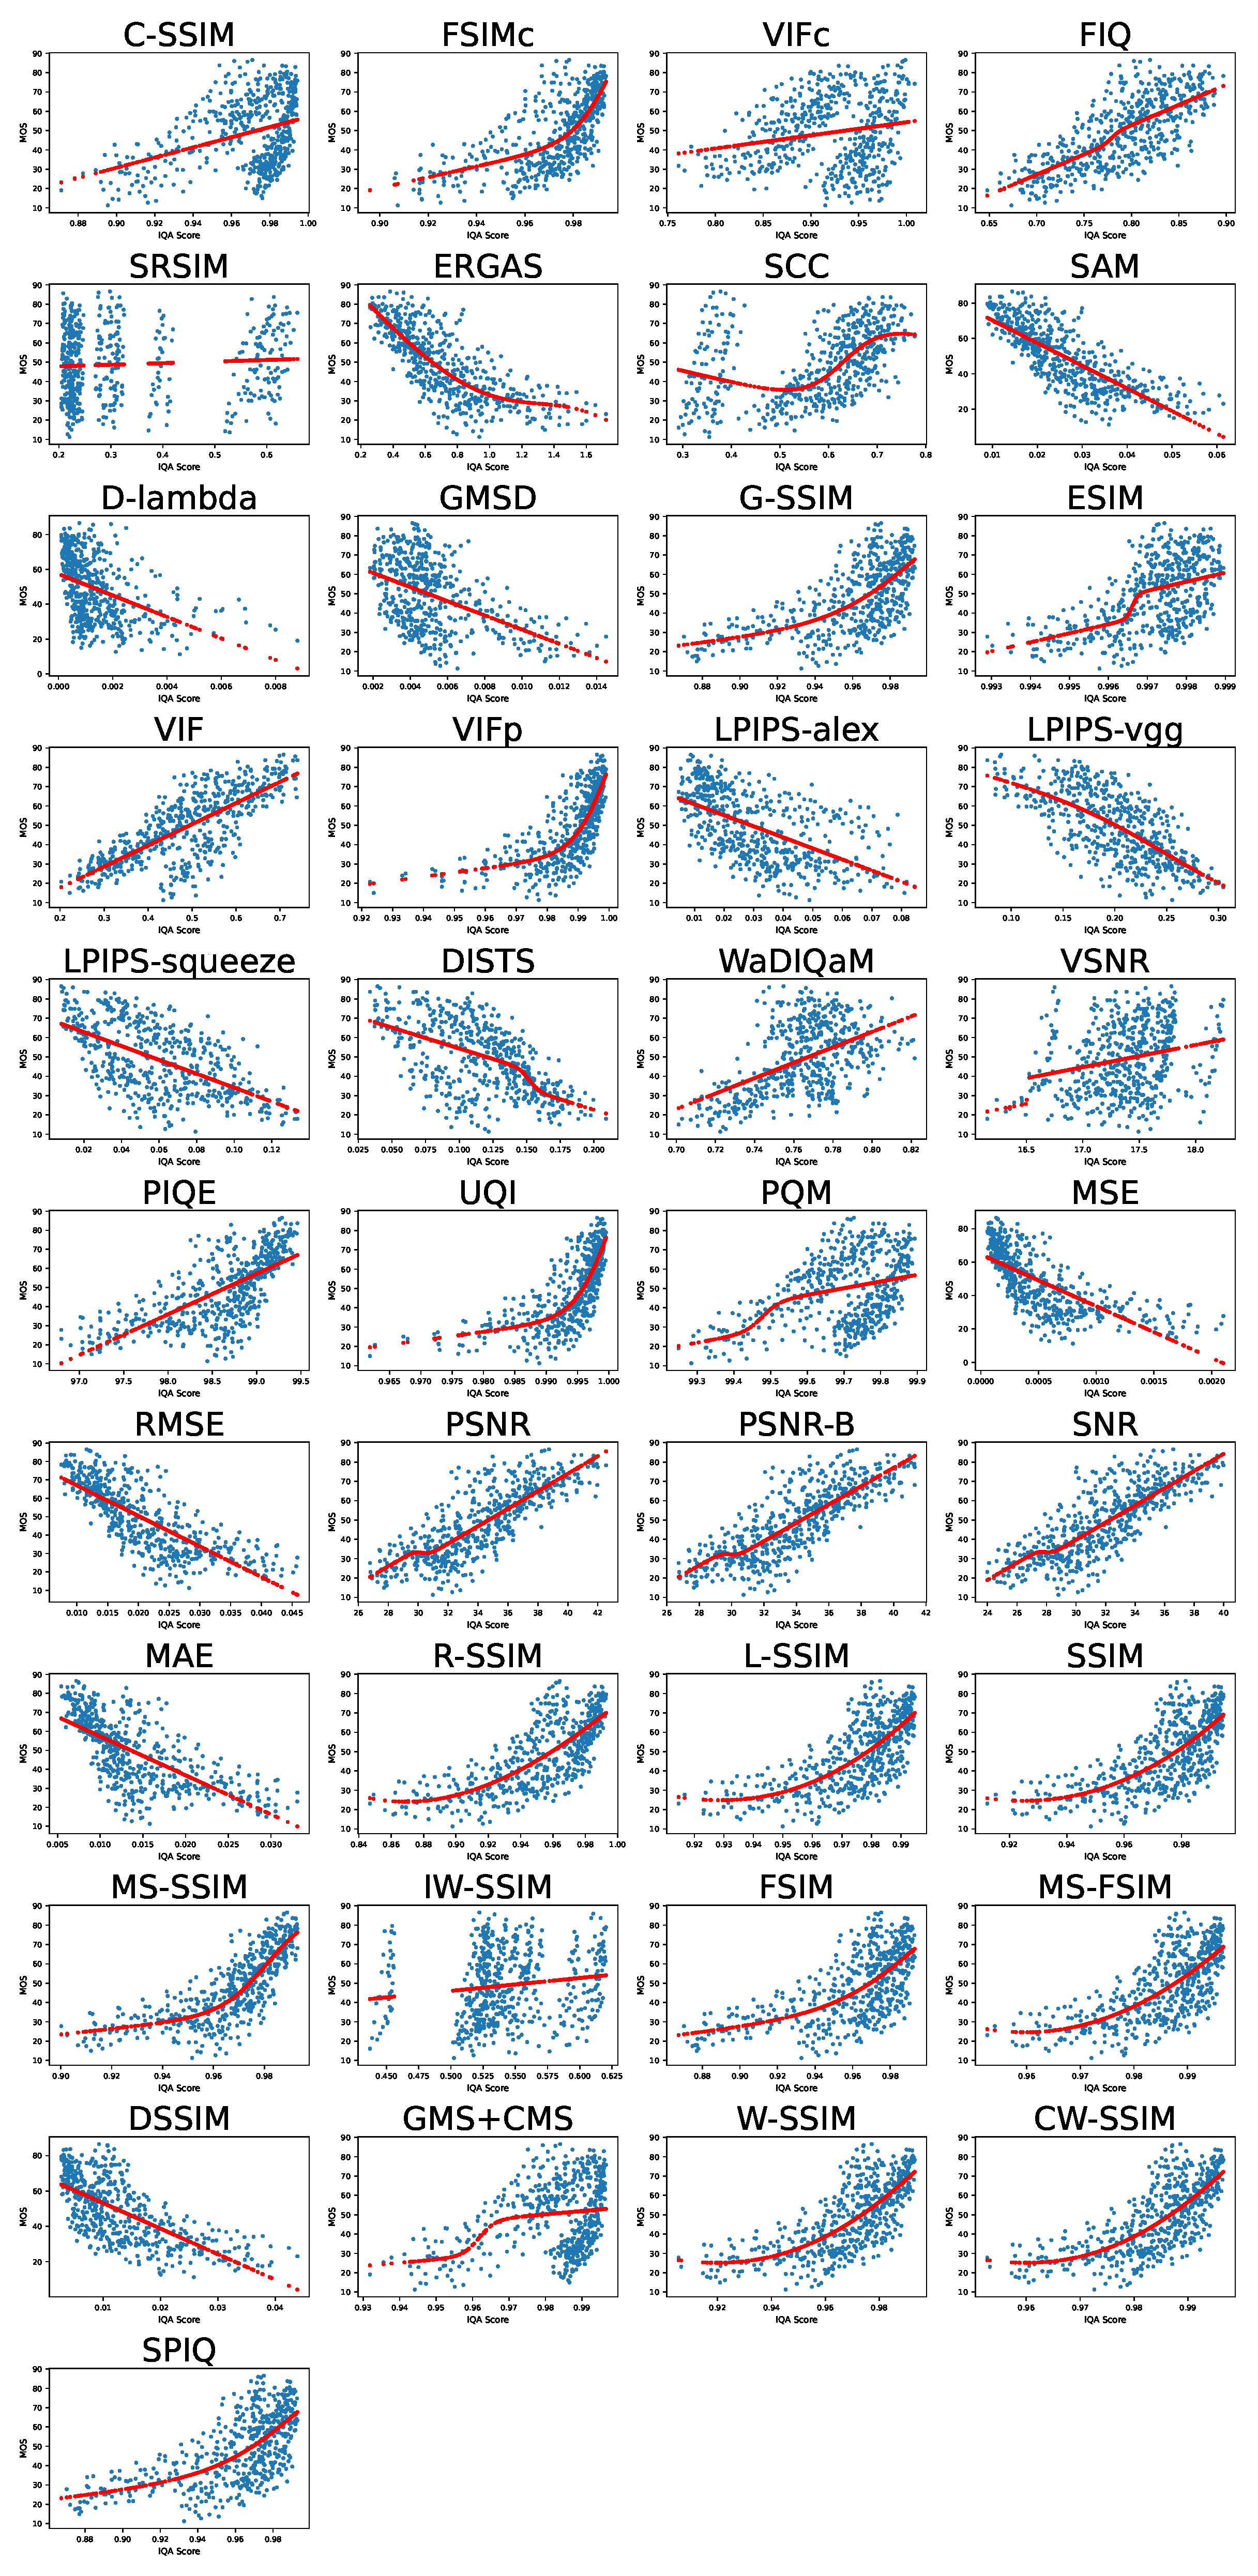
\includegraphics[width=0.7\linewidth]{images/mos_vs_iqa_grid.eps}
    \caption{Scatter plots illustrating the relationship between Mean Opinion Scores (MOS) and individual Full-Reference IQA metrics.}\label{fig:mos_vs_iqa}
\end{figure}

\begin{figure}
    \centering
    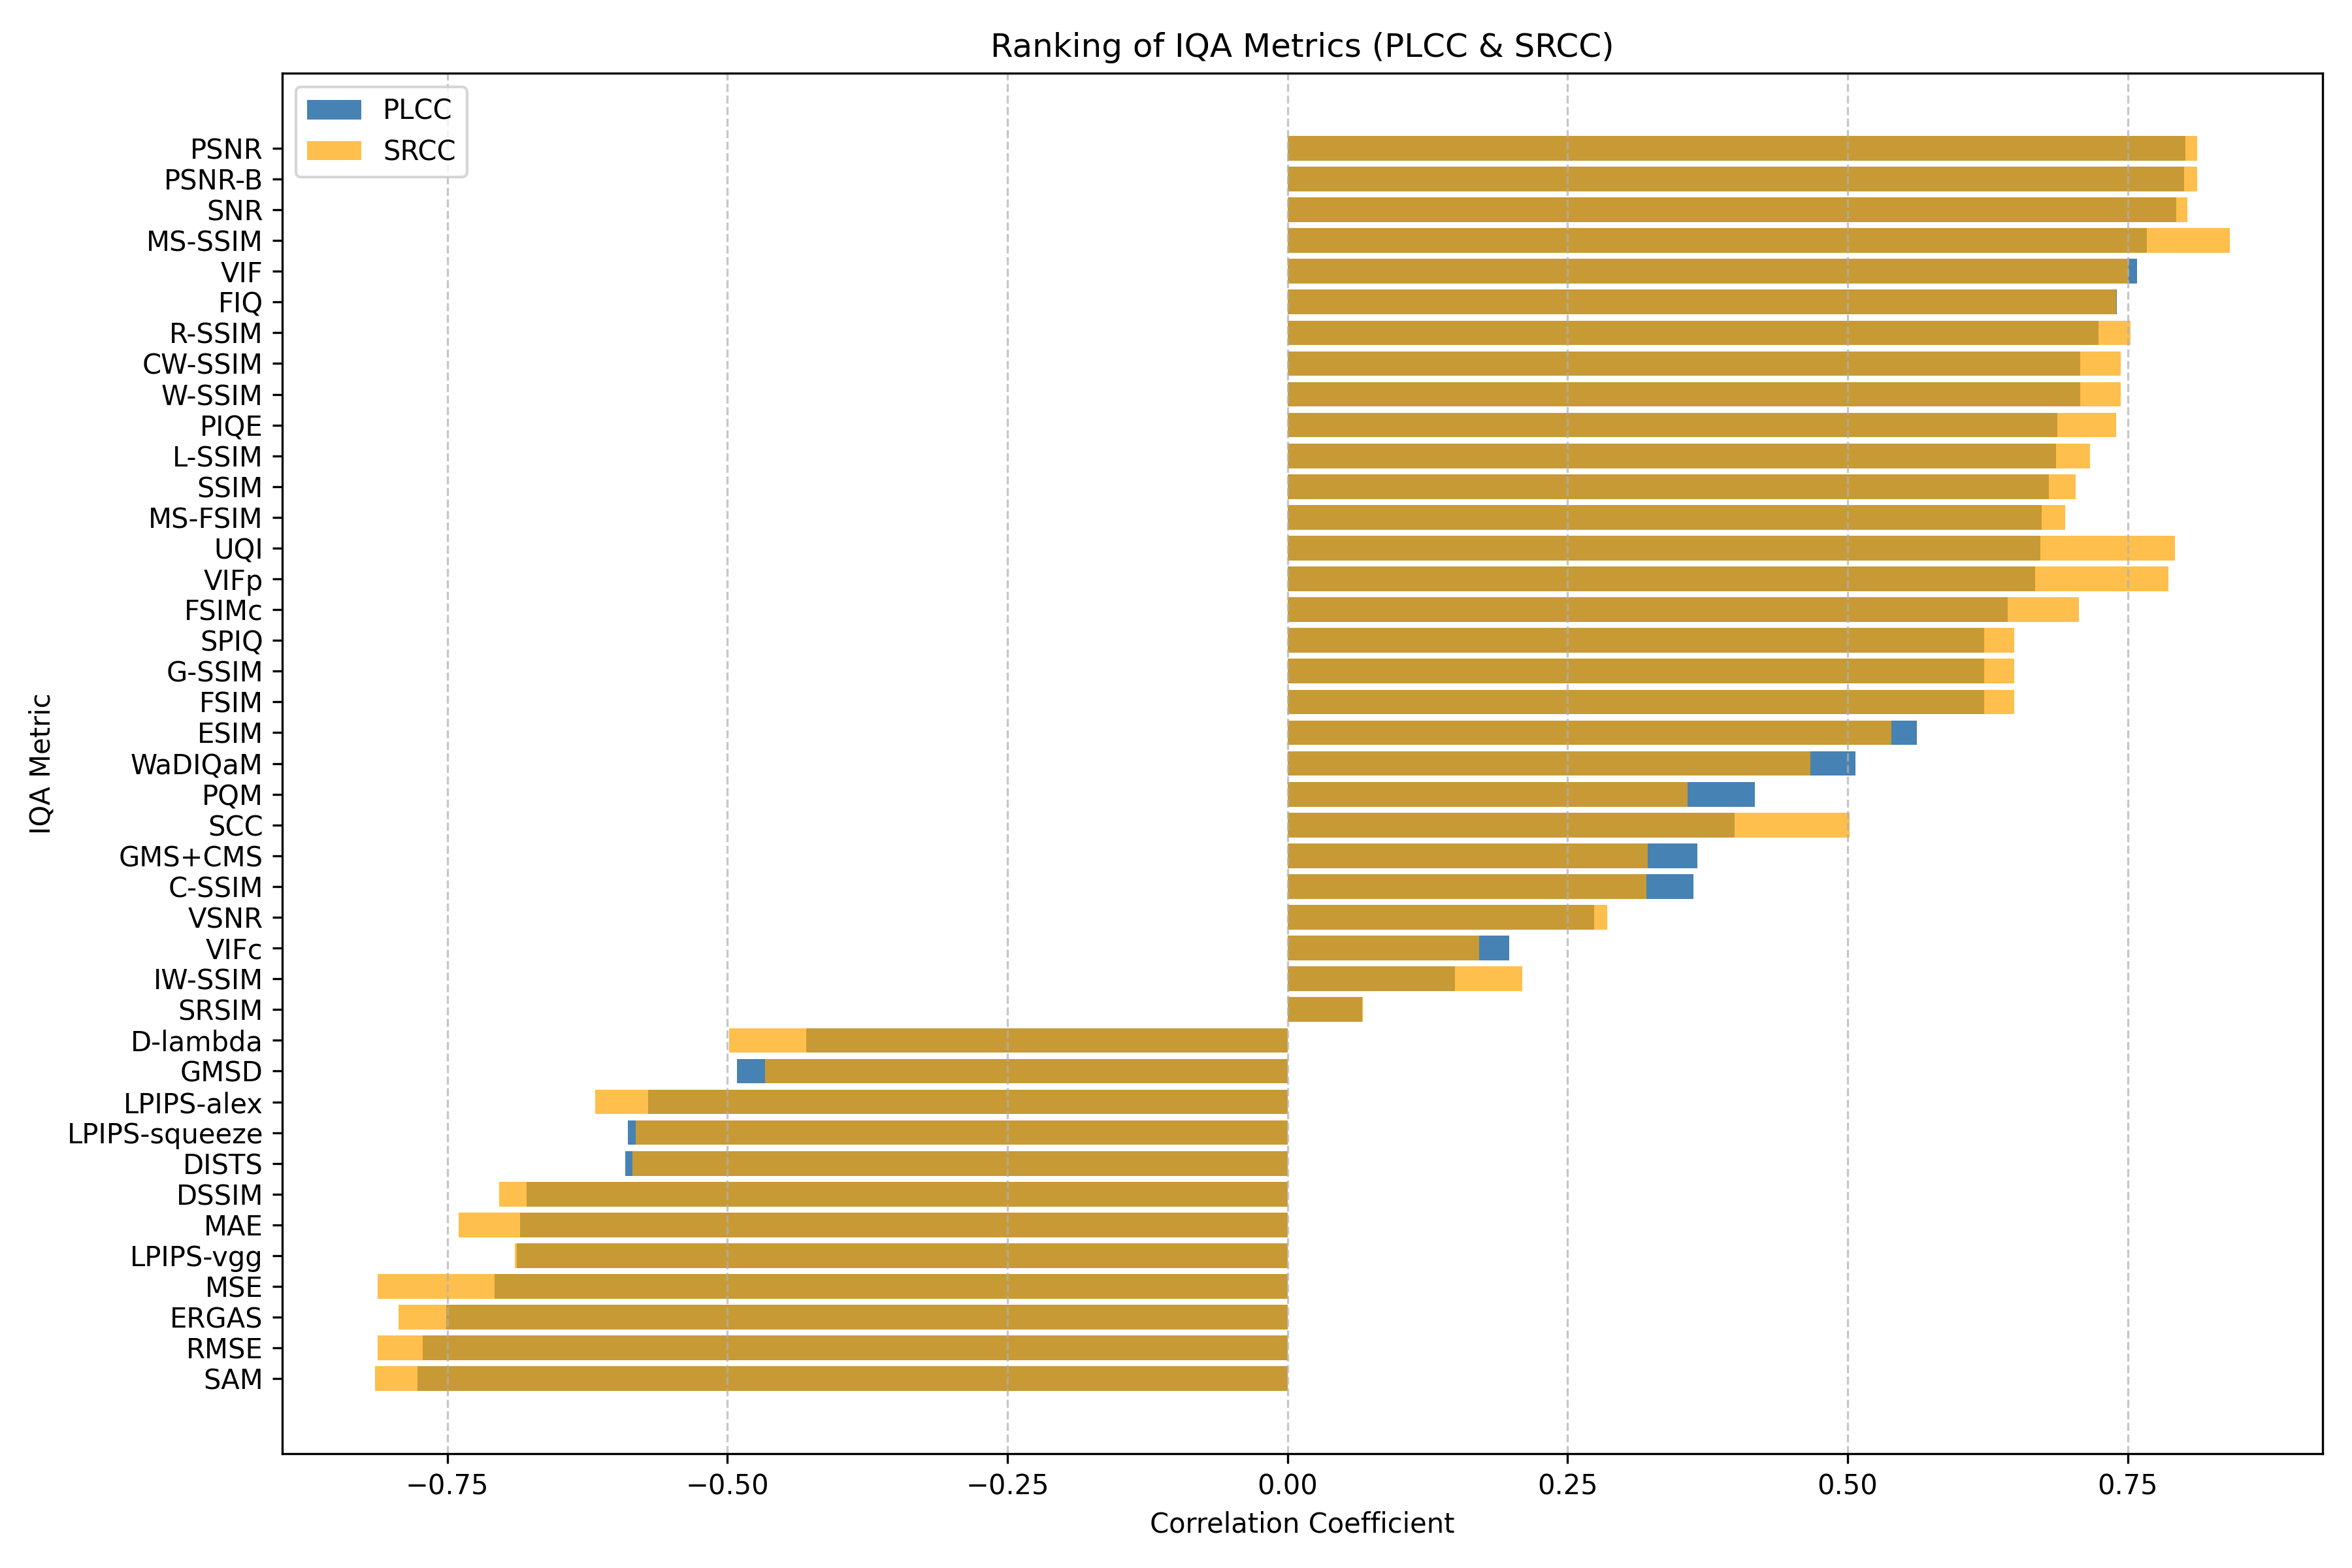
\includegraphics[width=0.9\linewidth]{images/metrics_bar.png}
    \caption{Ranking of FR-IQA metrics by correlation with MOS (PLCC and SRCC).}\label{fig:ranking}
\end{figure}

\subsection{Full-Reference Fusion Performance}

Using the 432 MOS-labeled images and $k = 5$ best metrics, we evaluated six fusion models.

As summarized in Table~\ref{tab:fusion_scores}, the Random Forest regressor achieved the best overall performance across all four evaluation metrics, as seen in Fig.~\ref{fig:randomforest}. Notably, it reached a PLCC of 0.8582 and SRCC of 0.8637, outperforming both linear and gradient boosting approaches.

\begin{figure}
    \centering
    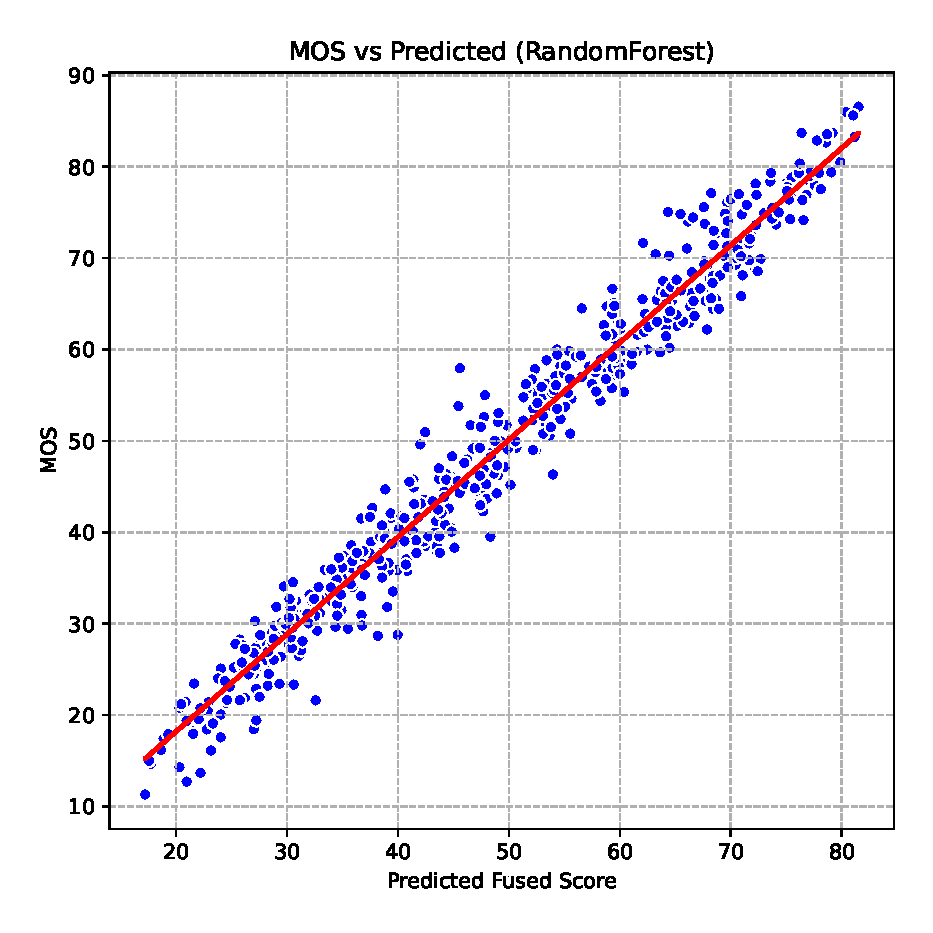
\includegraphics[width=0.6\linewidth]{images/fusion_plot_RandomForest.eps}
    \caption{MOS vs. Predicted fused Random Forest score}\label{fig:randomforest}
\end{figure}

\begin{table}
\caption{Fusion performance on 432 labeled images (MOS ground truth).}
\begin{center}
\begin{tabular}{lcccc}
\toprule
\textbf{Model} & \textbf{PLCC} & \textbf{SRCC} & \textbf{MSE} & \textbf{MAE} \\
\midrule
Linear Regression & 0.8123 & 0.8248 & 108.83 & 7.98 \\
Ridge             & 0.8125 & 0.8246 & 108.76 & 7.96 \\
Random Forest     & \textbf{0.8582} & \textbf{0.8637} & \textbf{84.48}  & \textbf{6.95} \\
SVR               & 0.8207 & 0.8207 & 108.44 & 8.08 \\
XGBoost           & 0.8560 & 0.8596 & 108.44 & 8.08 \\
LightGBM          & 0.8560 & 0.8577 & 85.90  & 7.15 \\
\bottomrule
\end{tabular}\label{tab:fusion_scores}
\end{center}
\end{table}

The trained Random Forest model was then applied to 3,132 unlabeled images, generating pseudo-MOS scores that serve as soft ground truth for the no-reference model.

\subsection{No-Reference Regression Model}

We trained a NR regressor using features extracted from a ResNet-18 pretrained on ImageNet. These features, paired with the pseudo-MOS scores generated from the fusion model, served as training data for a second Random Forest model.

Fig.~\ref{fig:nr_vs_fusion} shows the resulting alignment between the predicted NR quality scores and the fusion-based pseudo-MOS values. A clear linear trend is observed, with the model capturing both low and high quality regimes effectively.

\begin{figure}
    \centering
    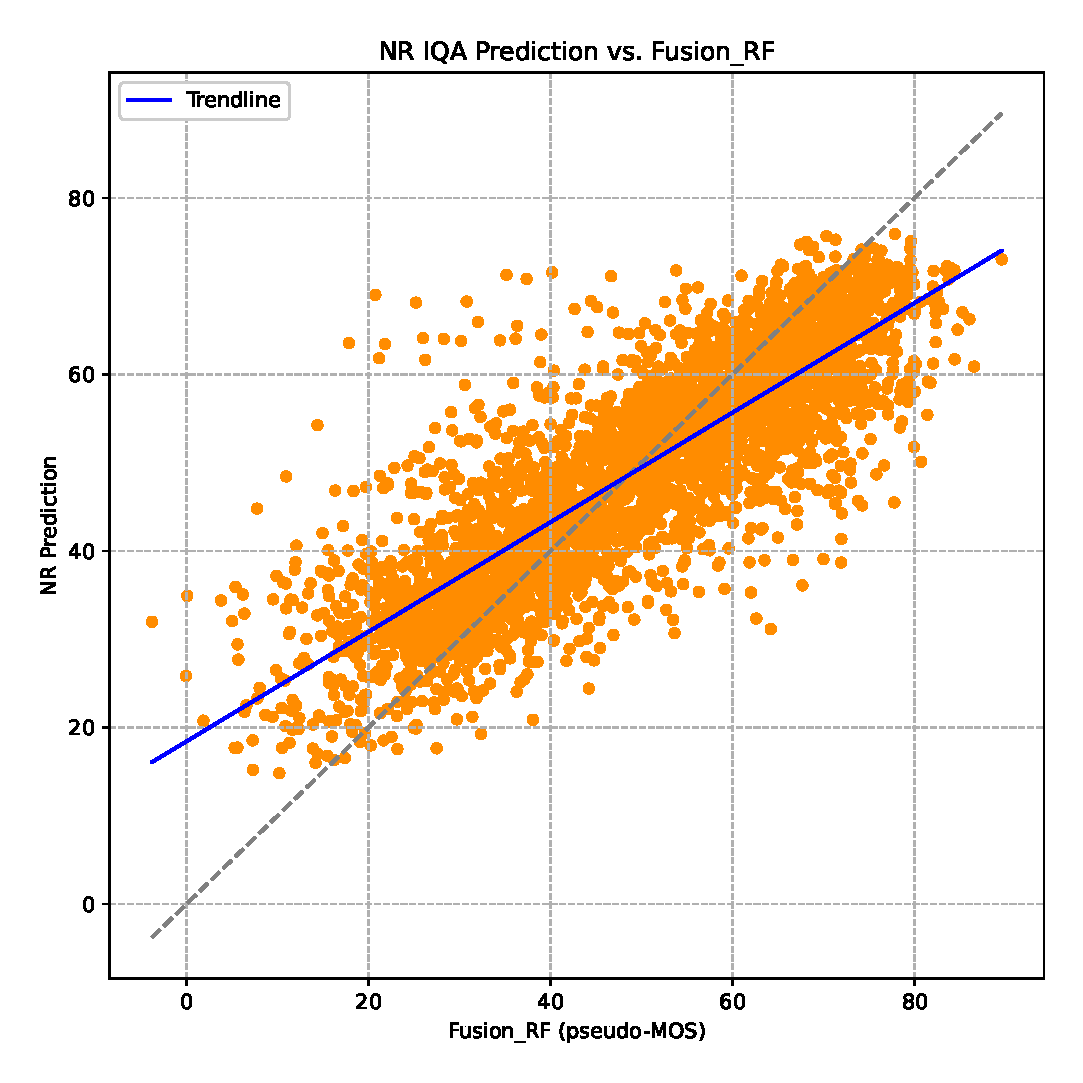
\includegraphics[width=0.6\linewidth]{images/nr_vs_fusion_rf.eps}
    \caption{Scatter plot of NR predictions vs.\ pseudo-MOS scores. The dashed line indicates identity; the blue line is the linear trend.}\label{fig:nr_vs_fusion}
\end{figure}

Quantitative results are reported in Table~\ref{tab:nr_scores}. Our proposed model, trained using deep features and pseudo-MOS supervision, achieves a PLCC of 0.8361 and SRCC of 0.8382, with an MSE of 90.48 and MAE of 7.16. In comparison, classical NR metrics such as NIQE and PIQE demonstrate weaker correlations with perceptual quality and substantially higher error. Even task-specific approaches like SER-FIQ and MagFace underperform, highlighting the robustness of our weakly supervised strategy for NR-IQA on steganographically degraded facial images.

\begin{table}
\caption{Performance of our NR IQA model, ResNet18 + Random Forest (RF), compared to standard NR-IQA baselines, using pseudo-MOS as ground truth.}
\begin{center}
\begin{tabular}{lcccc}
\toprule
\textbf{Method} & \textbf{PLCC} & \textbf{SRCC} & \textbf{MSE} & \textbf{MAE} \\
\midrule
Ours (ResNet18 + RF) & \textbf{0.8361} & \textbf{0.8382} & \textbf{90.48} & \textbf{7.16} \\
NIQE                 & 0.7536          & 0.7431          & 6859.81        & 82.62 \\
PIQE                 & 0.2993          & 0.3114          & 3297.65        & 57.05 \\
SER-FIQ              & -0.1648         & -0.1542         & 123.50         & 9.23 \\
MagFace              & -0.6095         & -0.6362         & 4437.91        & 66.24 \\
\bottomrule
\end{tabular}\label{tab:nr_scores}
\end{center}
\end{table}


\section{Conclusion and Future Work}

We proposed a Full-to-No-Reference framework for FIQA that predicts image quality in the absence of reference images by leveraging a pseudo-MOS supervision strategy. Our method first trains a FR fusion model to regress human perceptual judgments on a labeled subset (10\% of the dataset), generating pseudo-MOS labels for a larger unlabeled dataset. These forged labels are then used to train a deep NR regressor, enabling quality prediction from distorted images alone. This two-stage pipeline effectively bridges the gap between fully supervised FR-IQA and reference-free NR-IQA approaches.

Beyond the development of our NR IQA metric, the proposed framework offers a flexible foundation for constructing a variety of task-specific models. By enabling scalable, perceptually grounded supervision with limited ground-truth annotations, our approach can facilitate quality-aware training in applications such as GANs, forensic imaging, and domain-adapted biometric pipelines.

%---SAMPLE--
% REFERENCES
% Edit the references.bib file to add your own references, that you can then
\printbibliography\titleformat{\chapter}[display]	% Return chapter titles to normal, taking up a whole page (cool for appendices)
{\normalfont\huge\bfseries}{\chaptertitlename\ \thechapter}{20pt}{\Huge}


%APPENDIX
\begin{appendix}			% Start appendices
\chapter{Sample Appendix}\label{app: sample appendix}
\input{appendix/sample.tex}
% To include pdf use this
%\includepdf[pages={-}]{path/to/appendix.pdf}

\end{appendix}
\end{document}
